        %%******************************************%%
        %%                                          %%
        %%        Modello di tesi di laurea         %%
        %%            di Andrea Giraldin            %%
        %%                                          %%
        %%             2 novembre 2012              %%
        %%                                          %%
        %%******************************************%%

\begin{document}
    \frontmatter
    \begin{titlepage}
    \begin{center}
        \begin{LARGE}
            \textbf{\myUni}\\
        \end{LARGE}

        \vspace{10pt}

        \begin{Large}
            \textsc{\myDepartment}\\
        \end{Large}

        \vspace{10pt}

        \begin{large}
            \textsc{\myFaculty}\\
        \end{large}

        \vspace{30pt}
        \begin{figure}[htbp]
            \centering
            
\includegraphics[height=6cm]{unipd-logo}
        \end{figure}
        \vspace{30pt}

        \begin{LARGE}
            \textbf{\myTitle}\\
        \end{LARGE}

        \vspace{10pt}

        \begin{large}
            \textsl{\myDegree}\\
        \end{large}

        \vspace{40pt}

        \begin{large}
            \begin{flushleft}
                \textit{Relatore}\\
                \vspace{5pt}
                \profTitle\ \myProf
            \end{flushleft}

            % You can tweak the spacing to have professor and student names on the same line
            % useful if the page is broken by a long thesis title and you need more space
            % \vspace{-52pt}

            \begin{flushright}
                \textit{Laureando}\\
                \vspace{5pt}
                \myName
            \end{flushright}
        \end{large}

        \vspace{40pt}

        \line(1, 0){338} \\
        \begin{normalsize}
            \textsc{Anno Accademico \myAA}
        \end{normalsize}
    \end{center}
\end{titlepage}

    \clearpage
\phantomsection
\thispagestyle{empty}

\hfill
\vfill

\noindent\myName: \textit{\myTitle,}
\myDegree,
\textcopyright\ \myTime.

    %\cleardoublepage
\phantomsection
\thispagestyle{empty}
\pdfbookmark{Dedica}{Dedica}

\vspace*{3cm}

\begin{center}
    Lorem ipsum dolor sit amet, consectetuer adipiscing elit. \\ \medskip
    --- Oscar Wilde
\end{center}

\medskip

\begin{center}
    Dedicato a ...
\end{center}

    \cleardoublepage
\phantomsection
\pdfbookmark{Summary}{Summary}
\begingroup
\let\clearpage\relax
\let\cleardoublepage\relax
\let\cleardoublepage\relax

\chapter*{Summary}

The following documents describes the work done during the internship period, lasting about three hundred hours, by the student Marco Bernardi at the company Breton S.p.A.\\
There were several objectives to be achieved.\\
First of all, the feasibility study of the use of Generative Adversarial Networks to generate realistic marble textures was required.\\
Noted the feasibility, the second objective was to create a model that could generate marble textures with a high degree of realism and variability.\\
The third and final objective was the integration of the model in basic software for the creation of marble textures.\\

%\vfill

%\selectlanguage{english}
%\pdfbookmark{Abstract}{Abstract}
%\chapter*{Abstract}

%\selectlanguage{italian}

\endgroup

\vfill

    %\cleardoublepage\phantomsection\pdfbookmark{Acknowledgements}{acknowledgements}

\begin{flushright}{
    \slshape
    ``Life is really simple, but we insist on making it complicated''} \\
    \medskip
    --- Confucius
\end{flushright}


\bigskip

\begingroup
\let\clearpage\relax
\let\cleardoublepage\relax
\let\cleardoublepage\relax

\chapter*{Acknowledgements}

\noindent \textit{I want to thank \myProf, my thesis supervisor, for the support and patience he has shown me throughout my thesis.}
\noindent \textit{I would also like to thank my cat \textbf{mimì} for the support, the great help and for being close to me at all times during the years of study.}
\noindent \textit{Finally, thanks to all my economic supporters}
\bigskip
\noindent\textit{\myLocation, \myTime}
\hfill\myName\endgroup

    \cleardoublepage
\pdfbookmark{\contentsname}{tableofcontents}
\setcounter{tocdepth}{2}
\tableofcontents
%\markboth{\contentsname}{\contentsname}
\clearpage

\begingroup
    \let\clearpage\relax
    \let\cleardoublepage\relax
    \let\cleardoublepage\relax

    % Figures list
    \phantomsection
    \pdfbookmark{\listfigurename}{lof}
    \listoffigures

    \vspace*{8ex}

    % Tables list
    \phantomsection
    \pdfbookmark{\listtablename}{lot}
    \listoftables

    \vspace*{8ex}
\endgroup

\cleardoublepage

    \cleardoublepage

    \mainmatter
    \chapter{Introduction}\label{cap:Introduction}
\section{The company}
Breton S.p.A is an Italian company specialized in the design, engineering and production of machinery and advanced systems for various industries. 
Established in 1963 by Marcello Toncelli, Breton gained international recognition as a leader in the production of cutting-edge industrial equipment. 
The company's headquarters are located in Castello di Godego, Italy, with numerous production facilities and branches strategically located around the world. 
Breton's experience spans multiple industries, including stone working, metal working, aerospace, automotive and more.
Their extensive product portfolio includes a wide variety of machinery, catering for the needs of both small workshops and large industrial companies.
With a strong focus on research and development, Breton has been instrumental in driving advances in automation and digitization within various industries.
The company constantly invests in cutting-edge technologies such as the artificial intelligence, Internet of Things (\gls{iotg}\glsfirstoccur) and machine learning to provide cutting-edge solutions to its customers. 
Also, Breton places a significant emphasis on sustainability and environmentally friendly practices. 
Through the development of energy efficient machinery, waste reduction initiatives and the promotion of sustainability production processes, Breton actively contributes to a greener and more sustainable environment future.
\subsection{Products and Services}
\subsubsection{Products}
Breton's product portfolio encompasses a wide range of machinery, including:
\begin{itemize}
    \item \textbf{CNC machines:} Breton's \gls{cncg}\glsfirstoccur machines are designed to provide high precision and accuracy in machining operations. The company offers a wide range of \gls{cncg} machines, including vertical machining centers, horizontal machining centers, and 5-axis machining centers.
    \item \textbf{Cutting and shaping systems:} Breton's cutting and shaping systems are designed to provide high precision and accuracy in cutting and shaping operations. The company offers a wide range of cutting and shaping systems, including waterjet cutting systems, laser cutting systems, plasma cutting systems, and wire cutting systems.
    \item \textbf{Polishing equipment:} Breton's polishing equipment is designed to provide high precision and accuracy in polishing operations. The company offers a wide range of polishing equipment, including polishing machines, polishing robots, and polishing systems.
    \item \textbf{Robotic solutions:} Breton's robotic solutions are designed to provide high precision and accuracy in robotic operations. The company offers a wide range of robotic solutions, including robotic arms, robotic cells, and robotic systems.
    \item \textbf{Software:} Breton provides software solutions for the management of the productivity process, that can be fully integrated with the existing systems, for grant the best performance of the machinery and grant the control over the production plant.
\end{itemize} 
\subsubsection{Services}
Breton offers a wide range of services to its customers, including:
\begin{itemize}
    \item \textbf{Consulting:} Breton provides consulting services to its customers, helping them choose the right machinery for their needs. The company's experts analyze the customer's requirements and recommend the most suitable solutions.
    \item \textbf{Installation:} Breton's technicians install the machinery at the customer's site and ensure that it is functioning properly.
    \item \textbf{Training:} Breton offers training programs to its customers, teaching them how to operate the machinery and get the most out of it.
    \item \textbf{Maintenance:} Breton provides maintenance services to its customers, ensuring that the machinery is running smoothly and efficiently.
\end{itemize}
\subsection{Certifications}
Breton is continuously improving its products, services and workflows to meet the highest standards of quality, safety, and environmental protection. \\
The company is certified according to the following standards:
\begin{itemize}
    \item \textbf{ISO 9001:} Breton is certified according to the ISO 9001 standard, which specifies requirements for a quality management system.
    \item \textbf{ISO 14001:} Breton is certified according to the ISO 14001 standard, which specifies requirements for an environmental management system.
    \item \textbf{UNI INAIL ed. 2001:} Breton is certified according to the UNI INAIL ed. 2001 standard, which specifies requirements for a health and safety management system.
\end{itemize}
\section{The idea}
The concept originated from a request made by the company aiming to extract key characteristics of a marble slab, including its veins, texture, and colors, in order to automatically generate a digital representation, or fingerprint, of the slab. 
This digital fingerprint can be effectively created using a conventional machine learning (\gls{mlg}\glsfirstoccur) model. 
However, accurately teaching the model to distinguish between veins and other features in marble slabs poses significant challenges, as the veins can vary and the slabs themselves are not always flawless.

To address this issue, a substantial number of images depicting the veins' paths are required to train the model effectively. 
However, obtaining such images is often problematic for various reasons:
\begin{itemize}
    \item The company Breton primarily works with test slabs and thus lacks a large collection of images.
    \item Depending on customers for image contributions is not always feasible, as they may be unwilling to share their own images.
\end{itemize}
Manually extracting the veins' paths from images is an extremely time-consuming task that demands significant human resources. 
Consequently, the proposed solution involves creating a generative model capable of producing a substantial quantity of images that include the respective veins' paths. 
These generated images can then be utilized to train the machine learning model effectively.
\subsection{Side Idea}
Derived from the main concept, an ancillary idea emerged: the creation of a computer numerical control (\gls{cncg}\glsfirstoccur) program based on an image file. 
This would enable the recreation of veins on engineered stone slabs using a \gls{cncg} machine. 
However, implementing this idea presents considerable challenges, as converting an image file into a \gls{cncg} program is a complex task. 
A \gls{cncg} program consists of a sequence of instructions for the machine, while an image file is composed of a matrix of pixels.

Consequently, the ancillary idea was revised and transformed into the following: ``Generating a marble slab image from a computer-aided design (\gls{cadg}\glsfirstoccur) model``.
This approach proves more viable, as the \gls{cadg} model can be readily converted into a \gls{cncg} program, which in turn can be utilized to fabricate a marble slab.

To accomplish this, a generative adversarial network (\gls{gang}\glsfirstoccur) model is required. 
The \gls{gang} model must possess the ability to accurately reproduce colors, textures, and veins that adhere to the path defined by the \gls{cadg} model. 
This approach offers increased feasibility, as the \gls{cadg} model can be easily transformed into a \gls{cncg} program, enabling the subsequent production of a marble slab.

\section{Goals}\label{sec:goals}
The goals of the project can be categorized into three main categories denoted by the following letters:
\begin{itemize}
    \item\textbf{M:} Mandatory goals, which represent the primary objectives of the project and are explicitly required by the commissioning company.
    \item\textbf{D:} Desirable goals, which serve as secondary objectives for the project and are not essential for the commissioning company but can add value to the overall outcome.
    \item\textbf{O:} Optional goals, which are additional objectives for the project that may be pursued based on feasibility and available resources.
\end{itemize}
Each goal is assigned a unique code consisting of the category letter followed by a number that identifies the specific objective.
The goals are listed in the following table:
\begin{table}[H]
    \caption{Goals}\label{tab:goals}
    \centering
    \begin{tabularx}{\textwidth}{|c|X|c|}
        \hline
        \textbf{Code} & \textbf{Description} & \textbf{Category}\\
        \hline
        M1 & Get an analytic and multidisciplinary thought, thanks to the decomposition of the problem in sub-problems & M\\
        \hline
        M2 & Reach a level of autonomy in the management of the project, with synthesis and critical thinking of the problems & M\\
        \hline
        M3 & Quality on the production of technological artifacts and on the documentation & M\\
        \hline
        D1 & Development of a \gls{pocg}\glsfirstoccur for generating marble images with a \gls{gang} model or similar technology & D\\
        \hline
        D2 & Development of a \gls{pocg} for augmenting resolution of an image & D\\
        \hline
        D3 & Validation of the artifacts produced & D\\
        \hline
        O1 & First product engineering approaches developed & O\\
        \hline
        O2 & Product testing in a manufacturing production environment & O\\
        \hline
    \end{tabularx}
\end{table}
\section{Text structure}
\begin{description}
    \item[{\hyperref[cap:Introduction]{First chapter}}] 
    The first chapter introduce the company and its products and services.\\
    It also describes the idea of the project and the text structure.
    \item[{\hyperref[cap:process-methodologies]{Second chapter}}] The second chapter describes the process and the methodology used for the development of the project.
    \item[{\hyperref[cap:internship-desc]{Third chapter}}] Third chapter describes the internship experience, and how the project was planned and developed.
    \item[{\hyperref[cap:design-coding]{Fourth chapter}}] The fourth chapter describes how the project technologies were implemented for reach the objectives.
    \item[{\hyperref[cap:verification-validation]{Fifth chapter}}] The fifth chapter describes how the project was tested and validated.
    \item[{\hyperref[cap:conclusions]{Sixth chapter}}] The sixth chapter describes the conclusions of the project.
\end{description}

During the writing of this document, the following conventions were adopted:
\begin{itemize}
    \item acronyms, abbreviations and ambiguous or uncommon terms mentioned are defined in the glossary, located at the end of this document;
    \item for the first occurrence of the terms defined in the glossary, the following nomenclature is used: \emph{word}\glsfirstoccur;
	\item the terms that require further explanation like technical words are marked with a subscript \emph{italic};
\end{itemize}

    \chapter{Process and methodologies}
\label{cap:process-methodologies}

\intro{In this chapter, we delve into the comprehensive exploration of the technologies employed during the internship and their broader application.}
\section{GANs}
\label{sec:gans}
\begin{figure}[H]
    \centering
    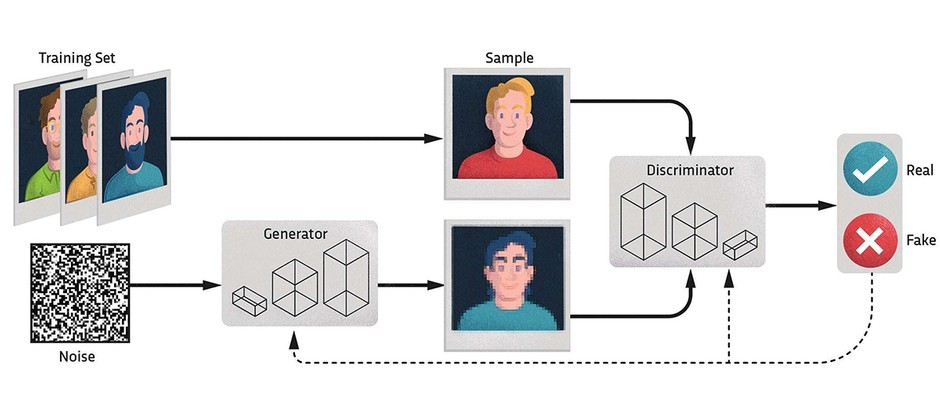
\includegraphics[width=0.75\textwidth]{images/model/gan-architecture}
    \caption{GAN architecture}\label{fig:gan-architecture}
\end{figure}

The concept of Generative Adversarial Networks (\gls{gang}) was first introduced by Ian Goodfellow and his colleagues in 2014 in their paper titled "Generative Adversarial Networks" \footcite{paper:ganpaper} published at the Neural Information Processing Systems (NIPS) conference. 
Goodfellow, along with his co-authors, proposed a novel framework that revolutionized the field of generative modeling. 
\gls{gang}s are a groundbreaking approach to generative modeling that combines elements of both supervised and unsupervised learning. 
They consist of two interconnected neural networks: a generator and a discriminator. 
The generator network learns to generate new data samples, such as images or text, by mapping random input vectors to output samples that resemble the training data. 
The discriminator network, on the other hand, aims to distinguish between real data samples from the training set and those generated by the generator. 
These two networks engage in a competitive process, where the generator strives to produce samples that the discriminator cannot differentiate from real data, while the discriminator aims to correctly classify the samples. (ref.~\ref{fig:gan-architecture}) 
Through iterative training, \gls{gang}s are able to improve the quality of the generated samples, leading to increasingly realistic and high-fidelity outputs. 
\gls{gang}s have since become a cornerstone in the field of generative modeling and have found applications in various domains, including image synthesis, text generation, and video generation. 



\section{Train process}
\label{sec:train-gan-model}
The training process of a \gls{gang} model involves a unique adversarial framework that iteratively improves the generator and discriminator networks. 
Initially, both networks are randomly initialized. During training, the generator takes random input vectors and generates synthetic data samples. 
Simultaneously, the discriminator receives both real data samples from the training set and generated samples from the generator. 
The discriminator's objective is to accurately distinguish between real and fake samples, while the generator aims to produce samples that can fool the discriminator into classifying them as real.
The training process occurs in alternating steps. In each step, the discriminator is trained by optimizing its parameters to minimize the classification error, correctly identifying real and generated samples. 
Conversely, the generator is trained by adjusting its parameters to maximize the error rate of the discriminator, essentially trying to generate samples that are indistinguishable from real data.
This adversarial game continues for multiple iterations, with the generator and discriminator networks continuously updating their weights to improve their performance. 
Through this iterative process, the generator learns to produce increasingly realistic samples, while the discriminator becomes more adept at distinguishing between real and generated data.
The training process of a \gls{gang} is complex and requires careful balancing. If the generator becomes too powerful, it may produce samples that closely resemble the training data but lack diversity. 
On the other hand, if the discriminator becomes too strong, it can easily detect generated samples, resulting in poor-quality outputs. Achieving a delicate equilibrium between the two networks is essential for training a successful \gls{gang} model.

\section{Evaluation process}
\label{sec:Evaluation-gan-model}
\subsection{The problem of evaluating GANs}
\label{subsec:problem-evaluating-gans}
In contrast to conventional deep learning models that are trained with a loss function until convergence, Generative Adversarial Networks (\gls{gang}s) operate within a zero-sum game framework involving two interconnected networks: the generator and the discriminator. 
The generator aims to deceive the discriminator by generating realistic samples, while the discriminator endeavors to accurately differentiate between genuine and fake samples. 
The training process concludes when the discriminator becomes incapable of distinguishing between real and synthetic samples, signifying that the generator has successfully captured the underlying distribution of the training data.

This unique training approach of \gls{gang}s poses a significant challenge when it comes to objective evaluation and assessment. 
Unlike traditional models that have objective functions to minimize or maximize, \gls{gang}s lack a definitive metric for gauging training progress and determining the absolute or relative performance of a \gls{gang} model solely based on loss. 
This presents several complexities in various scenarios, such as selecting a final \gls{gang} model during training, showcasing the capabilities of a GAN through generated samples, comparing different \gls{gang} models, or comparing different hyperparameters for the same \gls{gang} model.

To date, the most prevalent approach for evaluating \gls{gang}s involves a combination of qualitative and quantitative metrics that center around the quality and diversity of the generated samples.
\subsection{Manual evaluation}
\label{subsec:manual-evaluation}
Manual evaluation often serves as a means of assessing GAN models through the visual inspection of generated samples. 
This evaluation method relies on human judgment to gauge the quality of a batch of generated samples, rendering it subjective in nature. 
Although manual inspection is a straightforward approach to model evaluation, it entails several limitations. 
Firstly, subjectivity is introduced due to the evaluator's biases towards the model and the data. Secondly, expertise in the specific domain of the data is required to effectively evaluate the samples. 
Furthermore, manual evaluation is time-consuming, imposing constraints on the number of images that can be thoroughly assessed.

\emph{…evaluating the quality of generated images with human vision is expensive and cumbersome, biased […] difficult to reproduce, and does not fully reflect the capacity of models}
\footcite{paper:ganeval}.

Consequently, while manual evaluation provides an initial impression of a model's performance, it should not be solely relied upon for the final selection of a model. Fortunately, alternative and more objective evaluation methods have been proposed and embraced within the field.
\subsection{Qualitative evaluation}
\label{subsec:qualitative-evaluation}
Qualitative evaluation plays a crucial role in assessing the visual quality and performance of GAN models. 
While subjective in nature, it provides valuable insights into various aspects of the generated samples, including their fidelity, coherence, diversity, and novelty. 
Several commonly used metrics and evaluation techniques have been developed to facilitate qualitative assessment.
\begin{itemize}
    \item \textbf{Nearest neighbors}: Nearest neighbors evaluation involves comparing the generated samples with real samples from the training dataset. 
    By computing the similarity between the generated samples and their nearest neighbors in the real data space, evaluators can assess how well the GAN model captures the underlying distribution of the training data;
    \item \textbf{Rapid Scene Categorization}\footcite{paper:ganeval}: aims to evaluate the ability of GAN-generated samples to be quickly recognized and categorized by human observers. 
    Evaluators assess how well the generated samples align with the expected scene categories and their visual characteristics. This evaluation metric provides insights into the semantic coherence and overall discriminability of the generated samples;
    \item \textbf{Rating and Preference judgement}\footcite{paper:stackadvnet}\footcite{paper:stackadvnet1}\footcite{paper:stackadvnet2}\footcite{paper:stackadvnet3}:
    involve human evaluators rating or ranking the quality of generated samples based on predefined criteria. 
    This qualitative evaluation method provides subjective assessments of visual quality, realism, and aesthetic appeal. 
    By gathering ratings or preference judgments from multiple evaluators, a collective assessment of the generated samples can be obtained;
    \item \textbf{Mode Drop and Collapse}\footcite{paper:dropandcollapse}\footcite{paper:dropandcollapse2}: Mode drop and collapse refer to situations where the GAN model fails to generate samples representing all the diverse modes or aspects of the training data distribution. 
    Evaluators visually inspect the generated samples to identify any mode drop, where certain modes or patterns are missing, or mode collapse, where the generated samples lack diversity and exhibit repetitive patterns. 
    Assessing mode drop and collapse is crucial for evaluating the ability of GAN models to capture the full range of variations in the training data;
    \item \textbf{Network Internals}\footcite{paper:netint}\footcite{paper:netint1}\footcite{paper:netint2}\footcite{paper:netint3}\footcite{paper:netint4}\footcite{paper:netint5}: 
    Analyzing the internal representations and activations of the GAN model's neural network can provide insights into the learning process and the generated samples' quality. 
    Evaluators examine network internals, such as feature maps and intermediate layers, to gain a better understanding of how the GAN model generates and captures visual patterns;
\end{itemize}
The most used qualitative measure is a sort of manual inspection of images, called \emph{Rating and Preference judgement}.\\\\
\emph{\dots These types of experiments ask subjects to rate models in terms of the fidelity of their generated images\dots}\footcite{paper:ganeval}.\\\\
Usually images are shown in pairs (one real and one fake), and the subjects are asked to choose the best image.
A score or rating is then assigned to the model based on the number of times it is chosen as the best image.
For lowering the variance of the results, the images are shown to multiple human judges and the results are averaged.
This process is labor intensive, but with the help of crowd-sourcing platforms like Amazon Mechanical Turk, 
it can be done at scale (Reducing the cost also).\\
Another downside of this method is that the human judges performance can improve with experience, especially if they are given feedback on their performance.\\\\
\emph{\dots By learning from such feedback, annotators are better able to point out the flaws in generated images, giving a more pessimistic quality assessment\dots}\footcite{paper:ganeval}.\\\\
\subsection{Quantitative evaluation}
\label{subsec:quantitative-evaluation}
In addition to qualitative evaluation, quantitative assessment provides a systematic and objective analysis of GAN models' performance. 
These evaluation metrics aim to measure various aspects of the generated samples, including their diversity, fidelity, and similarity to the real data distribution. 
By quantitatively evaluating GAN models, researchers can compare different models, assess the impact of hyperparameters, and track progress during training.
Some of the most common quantitative measures are: Average log-likelihood, Coverage Metric, Inception Score, Modified Inception Score, Mode Score, AM Score, Fréchet Inception Distance, 
Maximum Mean Discrepancy, The Wasserstein Distance, Birthday Paradox Test, Classifier Two-Sample Tests, Classification Performance, Boundary Distortion, 
Number of Statistically-Different Bins, Image Retrieval Performance, Generative Adversarial Metric, Tournament Win Rate, Normalized Relative Discriminative Score, Adversarial Accuracy and Adversarial Divergence, 
Geometric Score, Reconstruction Score, Image Quality measures, Low-level Image Statistics, Precision, Recall and F1 Score.
%Quantitative measures are based on the use of metrics to evaluate the quality of the generated samples.
%All this methods use a numerical score to evaluate the quality.
%Some of the most common quantitative measures are: Average log-likelihood, Coverage Metric, Inception Score, Modified Inception Score, Mode Score, AM Score, Fréchet Inception Distance, Maximum Mean Discrepancy, The Wasserstein Distance, Birthday Paradox Test, Classifier Two-Sample Tests, Classification Performance, Boundary Distortion, Number of Statistically-Different Bins, Image Retrieval Performance, Generative Adversarial Metric, Tournament Win Rate, Normalized Relative Discriminative Score, Adversarial Accuracy and Adversarial Divergence, Geometric Score, Reconstruction Score, Image Quality measures, Low-level Image Statistics, Precision, Recall and F1 Score.\\
%%\begin{itemize}
%%    \item Average log-likelihood;
%%    \item Coverage Metric;
%%    \item Inception Score;
%%    \item Modified Inception Score;
%%    \item Mode Score;
%%    \item AM Score;
%%    \item Frechet Inception Distance;
%%    \item Maximum Mean Discrepancy;
%%    \item The Wasserstein Distance;
%%    \item Birthday Paradox Test;
%%    \item Classifier Two-Sample Tests;
%%    \item Classification Performance
%%    \item Boundary Distortion 
%%    \item Number of Statistically-Different Bins
%%    \item Image Retrieval Performance
%%    \item Generative Adversarial Metric
%%    \item Tournament Win Rate
%%    \item Normalized Relative Discriminative Score
%%    \item Adversarial Accuracy and Adversarial Divergence
%%    \item Geometric Score
%%    \item Reconstruction Score
%%    \item Image Quality measures
%%    \item Low-level Image Statistics
%%    \item Precision, Recall and F1 Score
%%\end{itemize}

The most used quantitative measures are \textbf{\emph{Inception Score}} and \textbf{\emph{Fréchet Inception Distance}}.
\subsubsection{Inception Score}
\label{subsubsec:inception-score}
The Inception Score (\gls{ISG}\glsfirstoccur) is a widely used quantitative metric for evaluating the quality and diversity of generated samples in \gls{gang} models.
It was proposed in 2016 by Tim Salimans et al. in \emph{"Improved Techniques for Training GANs"}\footcite{paper:salimans2016improved}, provides a measure of both sample quality and class diversity. 
The \gls{ISG} is computed by first obtaining the predicted class probabilities for each generated sample using an Inception-v3 pre-trained classifier. 
Then, the average of these probabilities is calculated to assess the quality of the generated samples. 
Additionally, the entropy of the predicted class probabilities is computed to measure the diversity of the samples. 
The formula for calculating the Inception Score is as follows:
\begin{equation}
    \label{eq:inception-score}
    \text{IS} = \exp \left( \mathbb{E}_{\mathbf{x} \sim p_{\text{data}}} \left[ \text{KL} \left( p(y|\mathbf{x}) || p(y) \right) \right] \right)
\end{equation}
The KL divergence is a measure of how one probability distribution is different from a second, reference probability distribution.
The KL divergence is defined as:
\begin{equation}
    \label{eq:kl-divergence}
    \text{KL}(P || Q) = \sum_{i} P(i) \log \left(\frac{P(i)}{Q(i)}\right)
\end{equation}
The Inception Score is a good measure of the quality of generated images, but it has some limitations.
It is sensitive to dataset and classifier choice, lacks consideration of spatial coherence, may not detect mode collapse effectively, offers limited interpretability, and emphasizes high-quality samples. 
Complementary metrics and qualitative assessments are essential for a comprehensive evaluation of GAN models.
\subsubsection{Frechet Inception Distance}
\label{subsubsec:frechet-inception-distance}
The Fréchet Inception Distance (\gls{fidg}\glsfirstoccur) score is a widely used metric for evaluating the quality of generated images in the field of generative adversarial networks (GANs) introduced by Martin Heusel et al. \footcite{paper:heusel2017gans}. 
\\\\
\emph{"FID performs well in terms of discriminability, robustness and computational efficiency [...] It has been shown that FID is consistent with human judgments and is more robust to noise than IS".}\footcite{paper:ganeval}\\\\
It measures the similarity between the distribution of real images and the distribution of generated images by comparing their feature representations extracted from a pre-trained Inception-v3 network\footcite{paper:inceptionv3}. 
A lower FID score indicates better similarity between the two distributions, suggesting higher-quality generated images that resemble the real data more closely. 
The FID score takes into account both the quality and diversity of generated images, making it a valuable metric for assessing the performance of GAN models. 
It provides a quantitative measure that complements visual inspection and subjective evaluation, enabling researchers to objectively compare and analyze different GAN architectures and training strategies.
The \gls{fidg} score is defined as:
\begin{equation}
    \label{eq:fid-score}
    \text{FID}(p, q) = \|\mu_p - \mu_q\|^2 + \text{Tr}(\Sigma_p + \Sigma_q - 2(\Sigma_p\Sigma_q)^{1/2})
\end{equation}
Where:
\begin{itemize}
    \item $\mu_p$ and $\mu_q$ are the mean vectors of the real and generated images respectively.
    \item $\Sigma_p$ and $\Sigma_q$ are the covariance matrices of the real and generated images respectively.
    \item \text{Tr} is the trace operator.
    \item $\|\cdot\|$ is the Euclidean norm.
\end{itemize}
As the \gls{ISG} score, the \gls{fidg} score has some limitations based on the use of the Inception-v3 network.
\subsubsection{Suggested GAN evaluation procedure}
\label{subsubsec:suggested-gan-evaluation-procedure}
The evaluation of Generative Adversarial Networks (\gls{gang}s) presents challenges, necessitating a comprehensive approach that combines qualitative and quantitative measures. 
Initially, a manual inspection of the generated images is recommended to assess the quality of the generator model. Subsequently, quantitative measures such as the Inception Score and the Frechet Inception Distance can be employed to evaluate the quality and diversity of the generated images. 
It is important to note that there is no universally superior measure for \gls{gang} evaluation, as the selection of evaluation measures depends on the specific task and dataset at hand.\\\\
\emph{
    As of yet, there is no consensus regarding the best score. Different scores assess various aspects of the image generation process, and it is unlikely that a single score can cover all aspects. Nevertheless, some measures seem more plausible than others (e.g. FID score)
}\footcite{paper:ganeval}
    \chapter{Internship description}\label{cap:internship-desc}
\intro{This chapter will describe the internship project, the requirements and the goals.}
\section{Initial analysis}
Given the idea of the project, the first step was to analyze the requirements for get a GAN model that was able to do the job.
Some questions were made to understand what we want to achieve and how to do it.
\begin{itemize}
    \item\textbf{What kind of images the model should generate?}
    \item\textbf{What kind of images the model should receive as input?}
    \item\textbf{What kind of network should be used?}
    \item\textbf{What kind of features should be extracted from the images?}
    \item\textbf{What kind of dataset should be used?}
\end{itemize}
From the previous questions, was possible to define Requirements, Goals and a road-map for the project.\\
\section{Requirements \& Goals}
\subsection{Requirements}
\begin{itemize}
    \item \textbf{Requirement 1}: The dataset should be composed by high quality images;
    \item \textbf{Requirement 2}: The model should be able to generate images from a given input, like a sketch;
    \item \textbf{Requirement 3}: The model should be able to generate images with a good quality, comparable with the real images;
    \item \textbf{Requirement 4}: The generated images should be previewed in real time;
\end{itemize}
\subsection{Goals}
\begin{itemize}
    \item \textbf{Goal 1}: Obtain a dataset of images with a good quality and variety;
    \item \textbf{Goal 2}: Obtain a model that is able to generate images from a sketch;
    \item \textbf{Goal 3}: Obtain a desktop application that is able to generate images in real time and preview them;
\end{itemize}
\section{Planning}
Initially, the project was planned using a story map~\ref*{label:story-map} to define the main features of the project and the main steps to achieve them.
\begin{figure}[H]
    \centering
    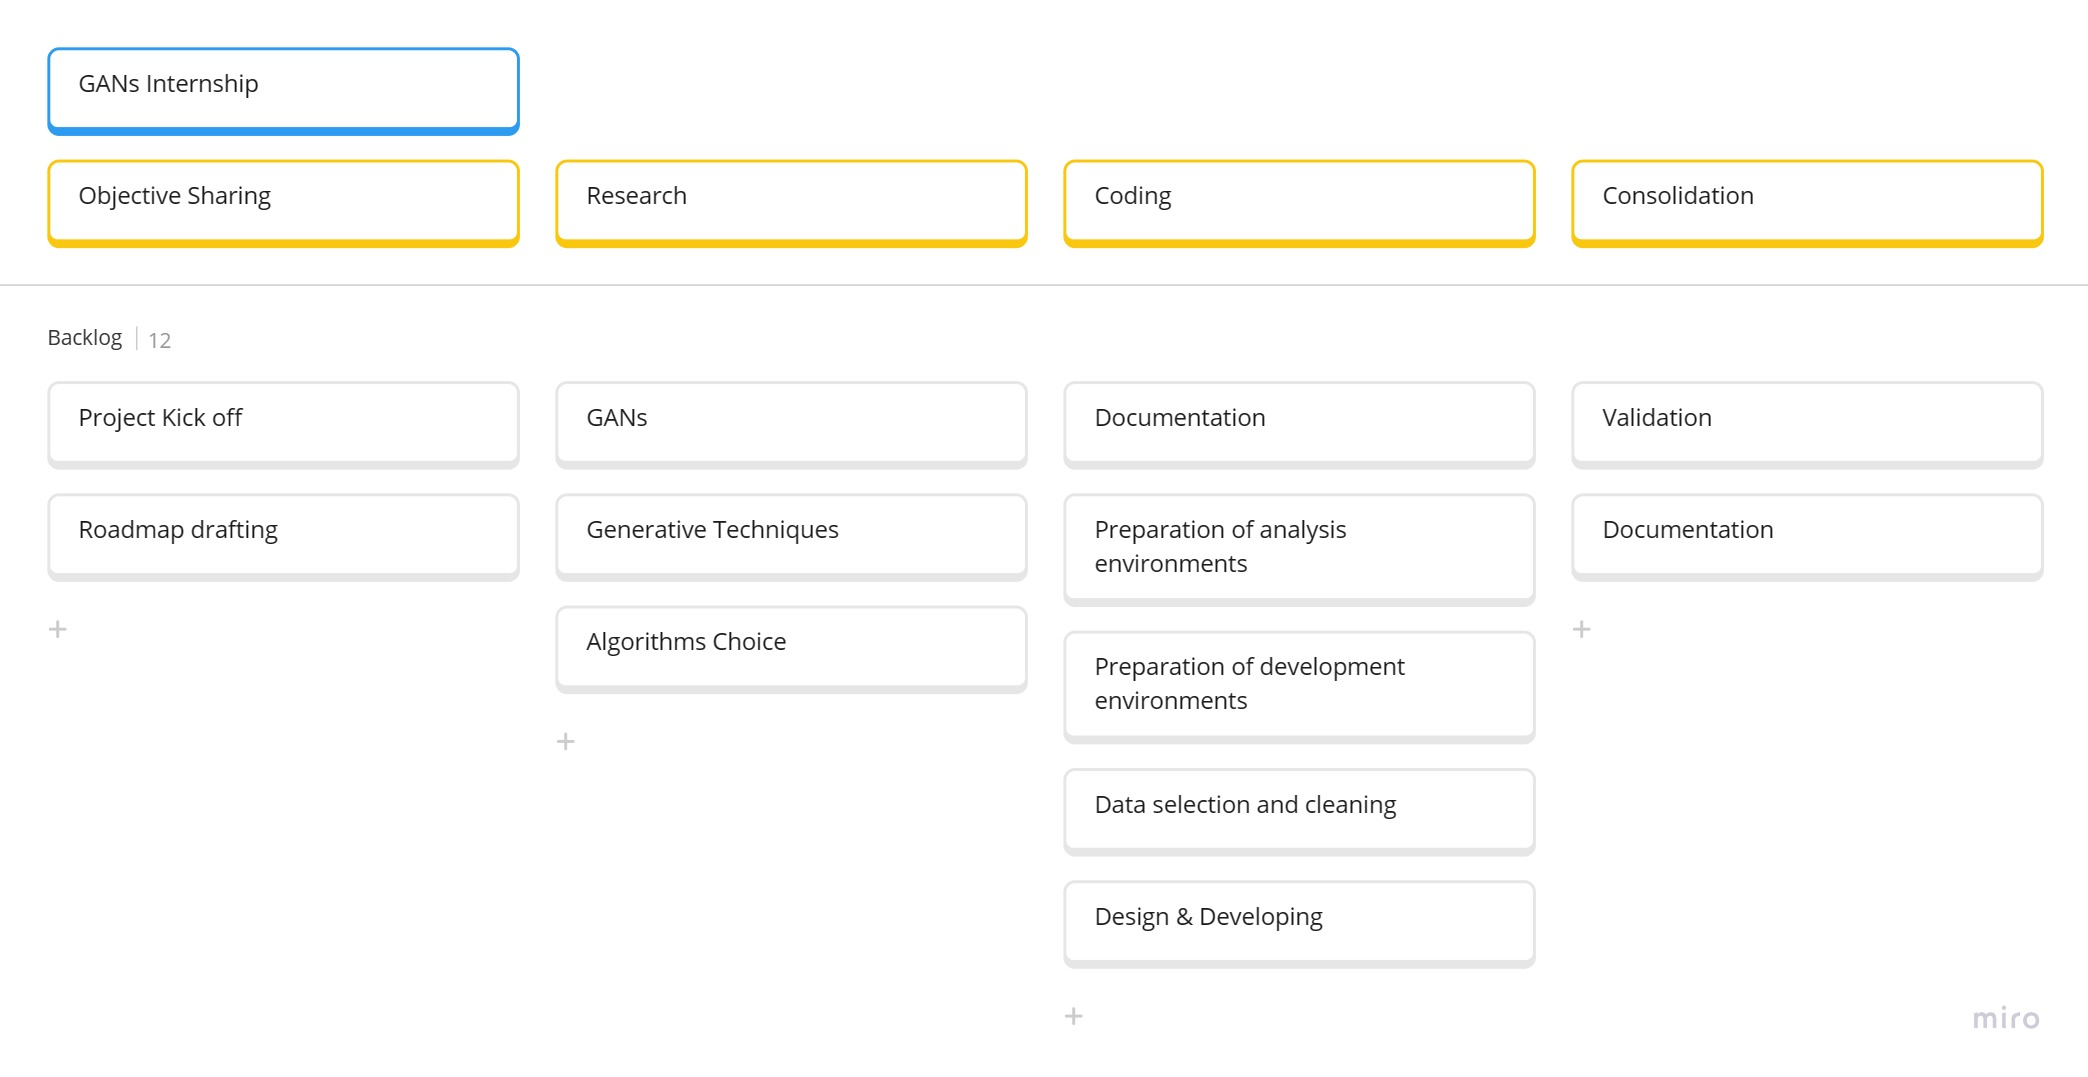
\includegraphics[width=1\textwidth]{images/story-map.jpg}
    \caption{Story map}\label{label:story-map}
\end{figure}
\subsection{Road-map}
After an Initial analysis of the story map, was possible to define a road-map for the project based on requirements and goals to achieve in the Internship period.
All the activity has been planned using a specific division of the time in different phases.
\begin{itemize}
    \item \textbf{Train period}: study of the state of the art and the technologies that will be used;
    \item \textbf{First period}: images acquisition;
    \item \textbf{Second period}: dataset increase, images augmentation;
    \item \textbf{Third period}: main feature extraction;
    \item \textbf{Fourth period}: network training;
    \item \textbf{Fifth period}: results analysis and improvement;
\end{itemize}
\begin{landscape}
\begin{ganttchart}[%Specs
    y unit title=0.5cm,
    y unit chart=0.6cm,
    x unit=1.0cm,
    vgrid,hgrid,
    title height=1,
%     title/.style={fill=none},
    title label font=\bfseries\footnotesize,
    bar/.style={fill=blue},
    bar height=0.7,
%   progress label text={},
    group right shift=0,
    group top shift=0.7,
    group height=.3,
    group peaks width={0.2},
    inline]{1}{12}
   %labels
   \gantttitle{Internship Project}{12}\\  % title 1           
   \gantttitle{April}{4}                      % title 3
   \gantttitle{May}{4}
   \gantttitle{June}{4}
   % Setting group if any
   \ganttgroup[inline=false]{Train Period}{2}{3}\\ 
   \ganttbar[progress=100,inline=false]{Technology exploration}{2}{3}\\

   \ganttgroup[inline=false]{First Period}{3}{4}\\ 
   \ganttbar[progress=100,inline=false]{Image acquisition}{3}{4}\\
   \ganttmilestone[inline=false]{Milestone 1}{4} \\

   \ganttgroup[inline=false]{Second Period}{3}{4}\\ 
   \ganttbar[progress=100,inline=false]{Dataset improvements}{3}{4}\\
   \ganttmilestone[inline=false]{Milestone 2}{4} \\

   \ganttgroup[inline=false]{Third Period}{4}{5}\\ 
   \ganttbar[progress=100,inline=false]{Features extraction}{4}{5}\\
   \ganttmilestone[inline=false]{Milestone 3}{5} \\

   \ganttgroup[inline=false]{Fourth Period}{5}{7}\\ 
   \ganttbar[progress=100,inline=false]{Network training}{5}{7}\\
   \ganttmilestone[inline=false]{Milestone 4}{7} \\

   \ganttgroup[inline=false]{Fifth Period}{7}{11}\\ 
   \ganttbar[progress=50,inline=false]{General improvements \& Docs}{7}{11}\\
   \ganttmilestone[inline=false]{Milestone 5}{11} \\
\end{ganttchart}
\end{landscape}
\subsection{Study Period:}
This period was used to study the state of the art and the technologies that will be used during the internship.\\
The main topics were:
\begin{itemize}
    \item \textbf{Machine Learning}: study of the main concepts of machine learning and deep learning;
    \item \textbf{GAN}: study of the main concepts of GAN and how they work;
    \item \textbf{GAN applications}: study of the main applications of GAN and how they are used;
    \item \textbf{GAN architectures}: study of the main GAN architectures and how they are used;
    \item \textbf{GAN training}: study of the main techniques used to train a GAN;\@
    \item \textbf{GAN evaluation}: study of the main techniques used to evaluate a GAN;\@
    \item \textbf{GAN improvements}: study of the main techniques used to improve a GAN;\@
    \item \textbf{GAN applications}: study of the main applications of GAN and how they are used;
\end{itemize}
\subsection{Train Period:}
During this was the acquisition of the images.
Every Breton machine has been equipped with a camera and a computer with a software that allows to acquire images from the camera.
This camera take a picture of each worked slab and send it to the database.
\subsubsection{Problems:}
The main problem in this phase was related to the quality of the images.
The images acquisition of the machine was not meant to be used for a machine learning project, so the quality of the images was not the best.
The images were not all of the same size and the background was not always the same, sometimes they contains reflections of the light or the shadow of the machine.
\subsubsection{Solutions:}
To solve this problems, some precautions were taken.
\begin{itemize}
    \item \textbf{Images background}: the background of the images was removed using a company previously trained \gls{mlg} model that was able to recognize the border of the slab.
                              With this model and OpenCV library it was possible to remove everything that was not the slab from the image.
    \item \textbf{Images defects}: the images contains light reflections and shadows was manually removed from the dataset.
                                   This was possible because the images were not too many.
    \item \textbf{Images size}: the images were resized to a common size, maintaining the aspect ratio.
\end{itemize}
\subsubsection{Milestone:}
At the end of the period the dataset was composed by 7000 images of slabs, with different colors and textures.
The dataset was divided in two parts, one for the training and one for the validation, with a ratio of 70\% and 30\% respectively.
\begin{figure}
    \centering
    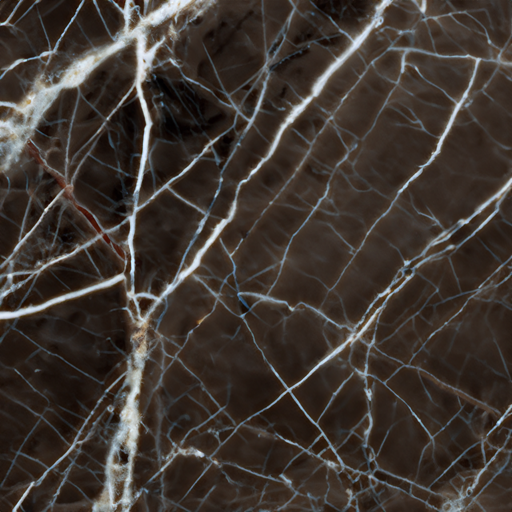
\includegraphics[height=6cm]{slabs/intera}
    \caption{Example of a slab}
\end{figure}
\subsection{Second Period:}
During this period the dataset was increased and the images were augmented.
\subsubsection{Augmentation:}
Augmentation is a technique that allows to increase the number of images in a dataset, applying some transformations to the original images.
This technique is useful when the dataset is not big enough to train a network.

The images augmentation technique applied was:
\begin{itemize}
    \item  \textbf{Resize}: each image was resized to a bigger size, from 256$\times$256 to 286$\times$286;
    \item  \textbf{Random Crop}: each image was randomly cropped to a size of 256$\times$256;
    \item  \textbf{Random Flip}: each image was randomly flipped horizontally;
\end{itemize}

For increasing the dataset, each original image was splitted in smaller images of 256$\times$256 pixels.

\subsubsection{Milestone:}

At the end of the period the dataset was composed by 7000 images of slabs, with different colors and textures.


\begin{figure}
    \centering
    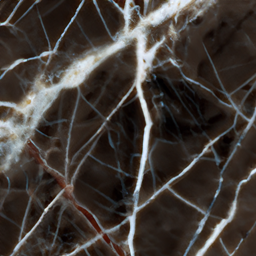
\includegraphics[width=.24\textwidth]{slabs/crop/crop_0_0}
    
\includegraphics[width=.24\textwidth]{slabs/crop/crop_0_1}
    \\
    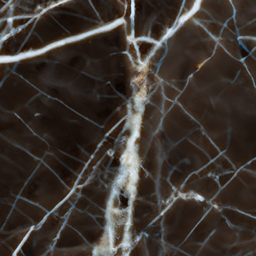
\includegraphics[width=.24\textwidth]{slabs/crop/crop_1_0}
    
\includegraphics[width=.24\textwidth]{slabs/crop/crop_1_1}
    \caption{Cropped image}\label{fig:foobar}
\end{figure}

\subsection{Third Period:}
This period was dedicated to found the best method to extract the features from the images. (Vein, texture, color, etc.)
Extracting the features from the images is the most important part of the project, because the quality of the features will affect the quality of the network.
So the mask that contains it must be as accurate as possible.

\subsubsection{Vein extraction:}
For the vein extraction, different Python implemented methods were tested.
The methods tested were:
\begin{itemize}
    \item \textbf{Threshold}\footcite{site:opencv-threshold}: this method is based on the Threshold algorithm.
    It consists in the application of a threshold to the image, so that only the pixels with a value higher than the threshold are kept.
    Setting a fixed threshold is not a good idea, because the images have different light conditions.
    So the threshold was calculated using the Otsu's method.
    \item \textbf{Canny Edge Detection}\footcite{site:opencv-canny}: this method is based on the homonym algorithm.
    The Canny algorithm is an edge detection algorithm that uses a multi-stage algorithm to detect a wide range of edges in images.
    The algorithm consists of 5 steps:
    \begin{enumerate}
        \item Noise reduction: the image is smoothed using a Gaussian filter;
        \item Gradient calculation: the intensity gradient of the image is calculated;
        \item Non-maximum suppression: the non-maximum suppression is applied to the gradient image;
        \item Double threshold: two thresholds are used to determine the edges;
        \item Edge tracking by hysteresis: the edges are tracked using the two thresholds.
    \end{enumerate}
    \begin{figure}[H]
        \centering
        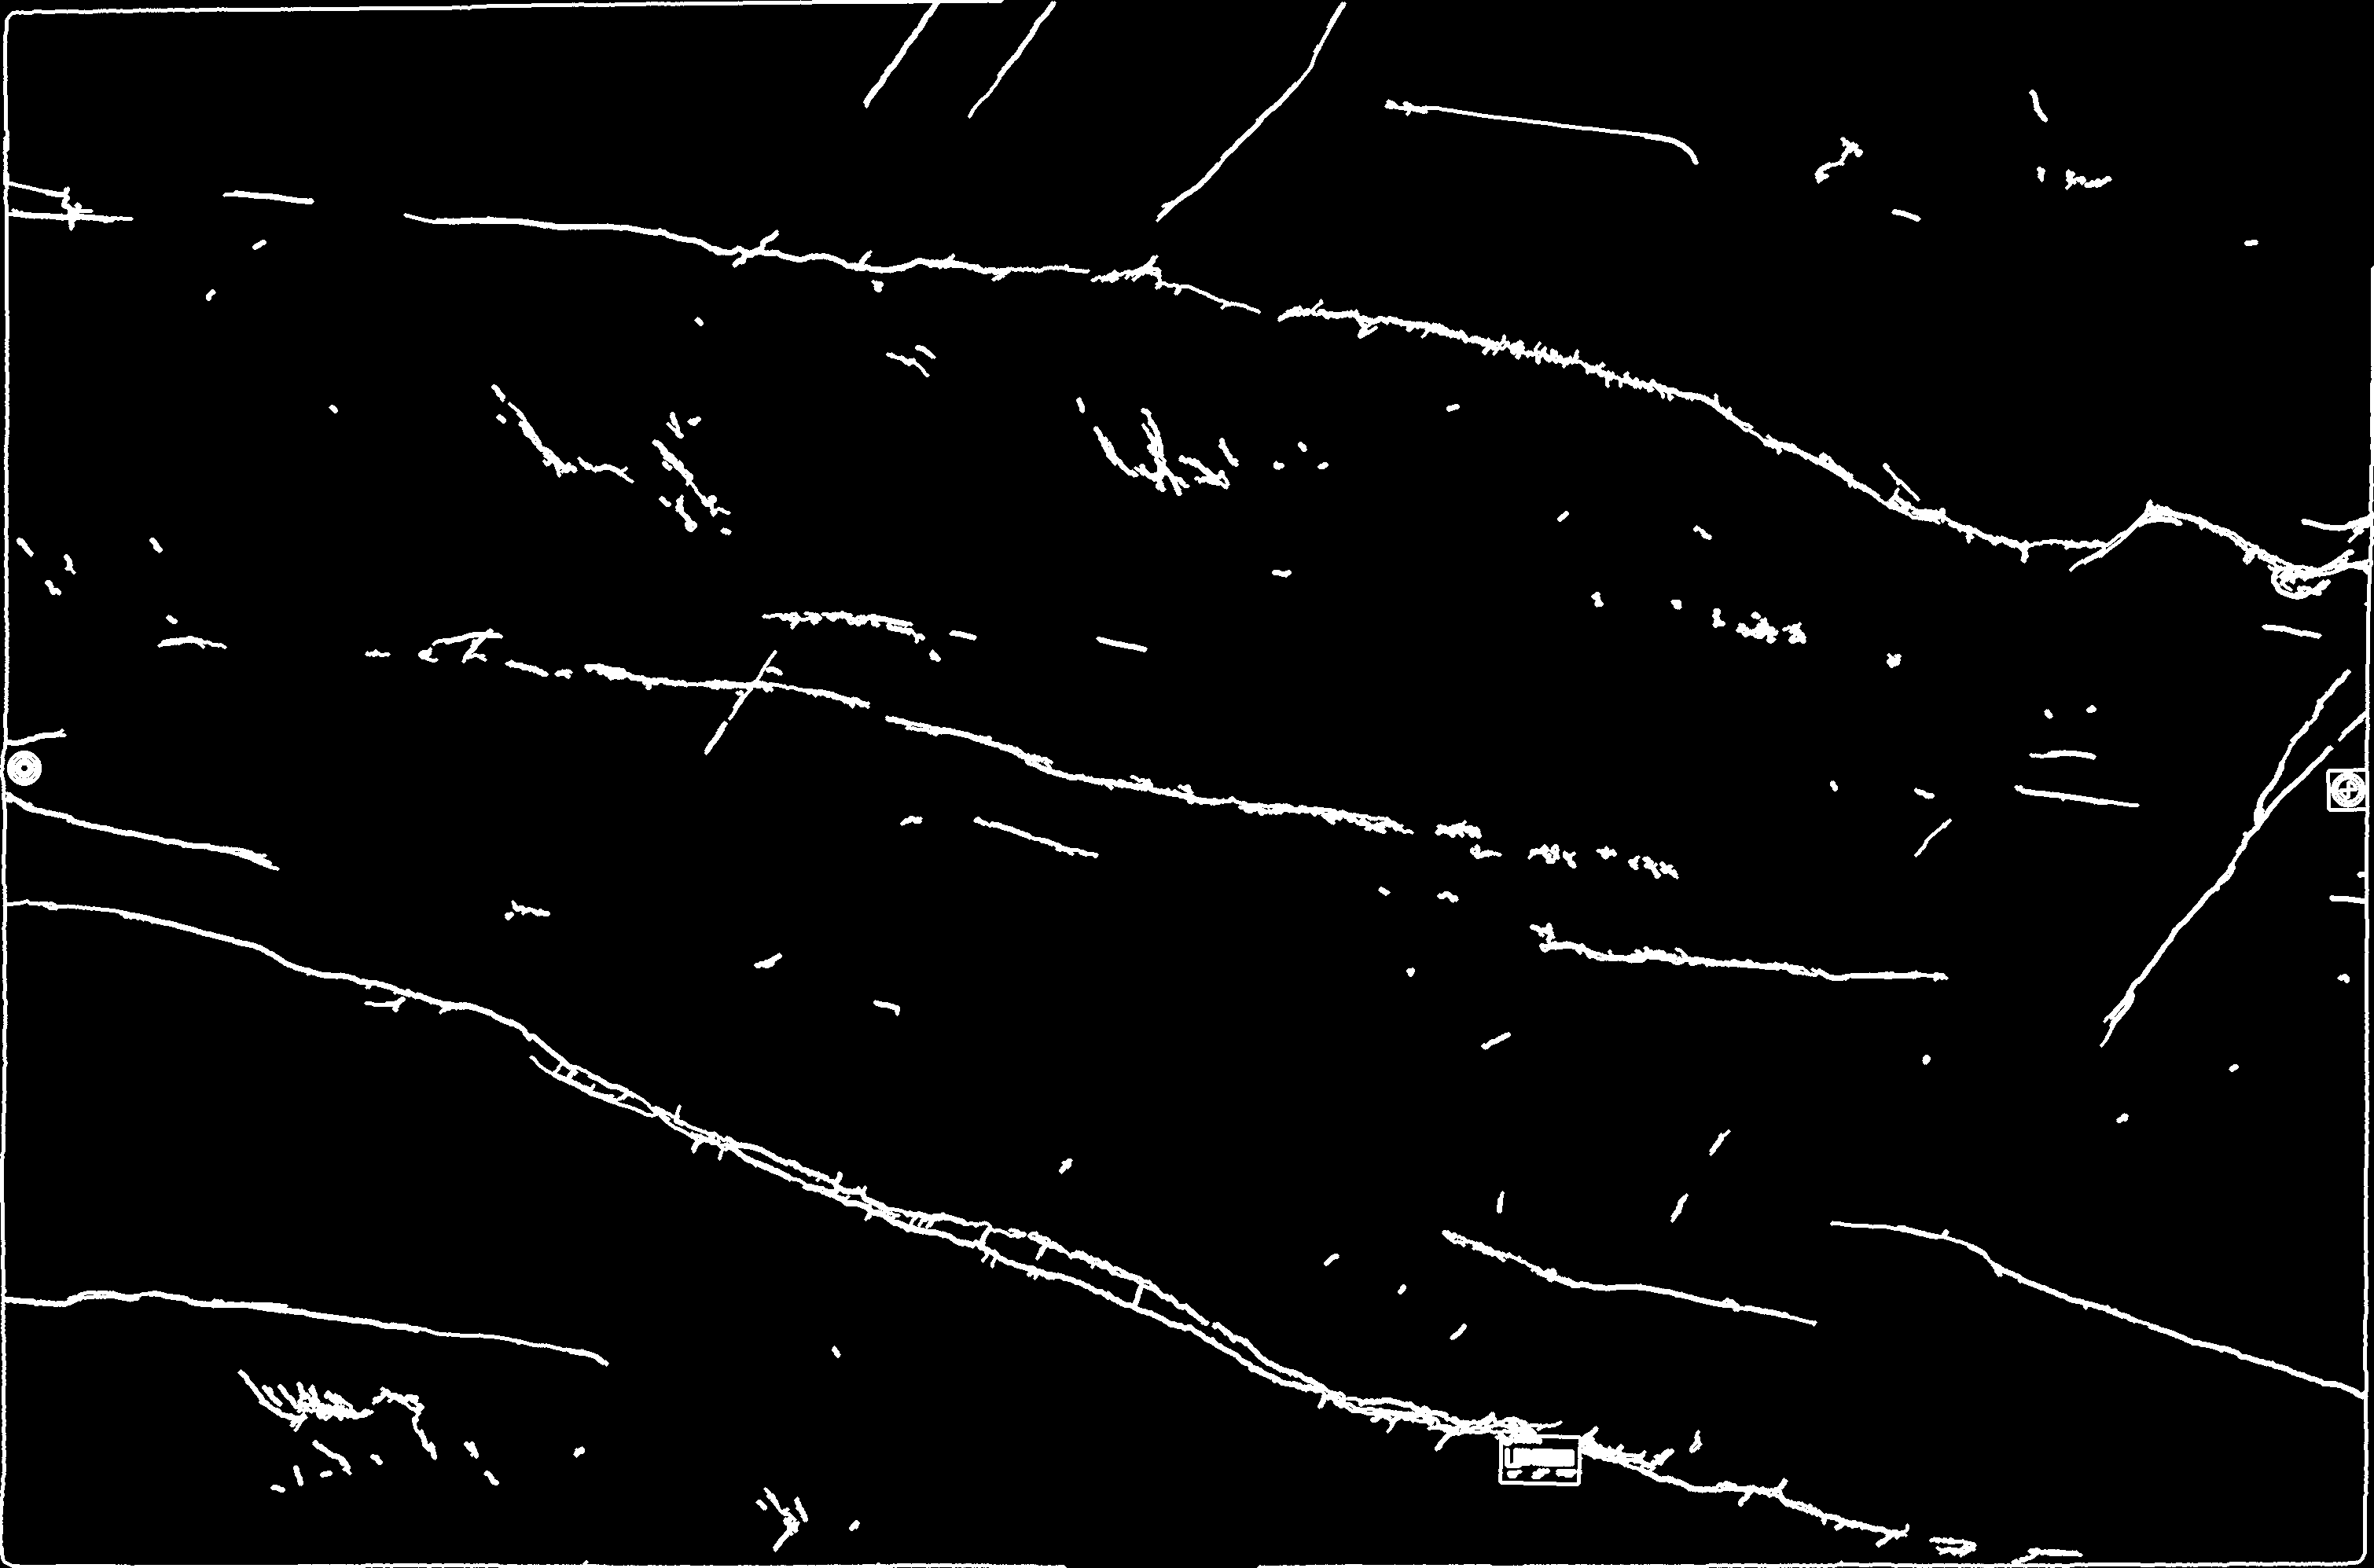
\includegraphics[width=.7\textwidth]{slabs/canny/canny}
        \\
        \includegraphics[width=.7\textwidth]{slabs/canny/canny_origin}
        \caption{Canny Edge Detection}\label{fig:canny_compare}
    \end{figure}
    In figure~\ref*{fig:canny_compare} is possible to see the result of the Canny Edge Detection.
    \item \textbf{Meijering \& Contrast filter}\footcite{site:sckit-meijering}: this method uses the Meijering filter to enhance the vein of the image.
    The Meijering filter is a filter that enhances the line-like structures in an image.
    It's based on the Hessian matrix, that is a square matrix containing the second order partial derivatives of a function.
    The Hessian matrix is used to calculate the eigenvalues and eigenvectors of the image.
    The eigenvalues are used to calculate the line-like structures of the image.
    The contrast filter is used to enhance the contrast of the image.
    \begin{figure}[H]
        \centering
        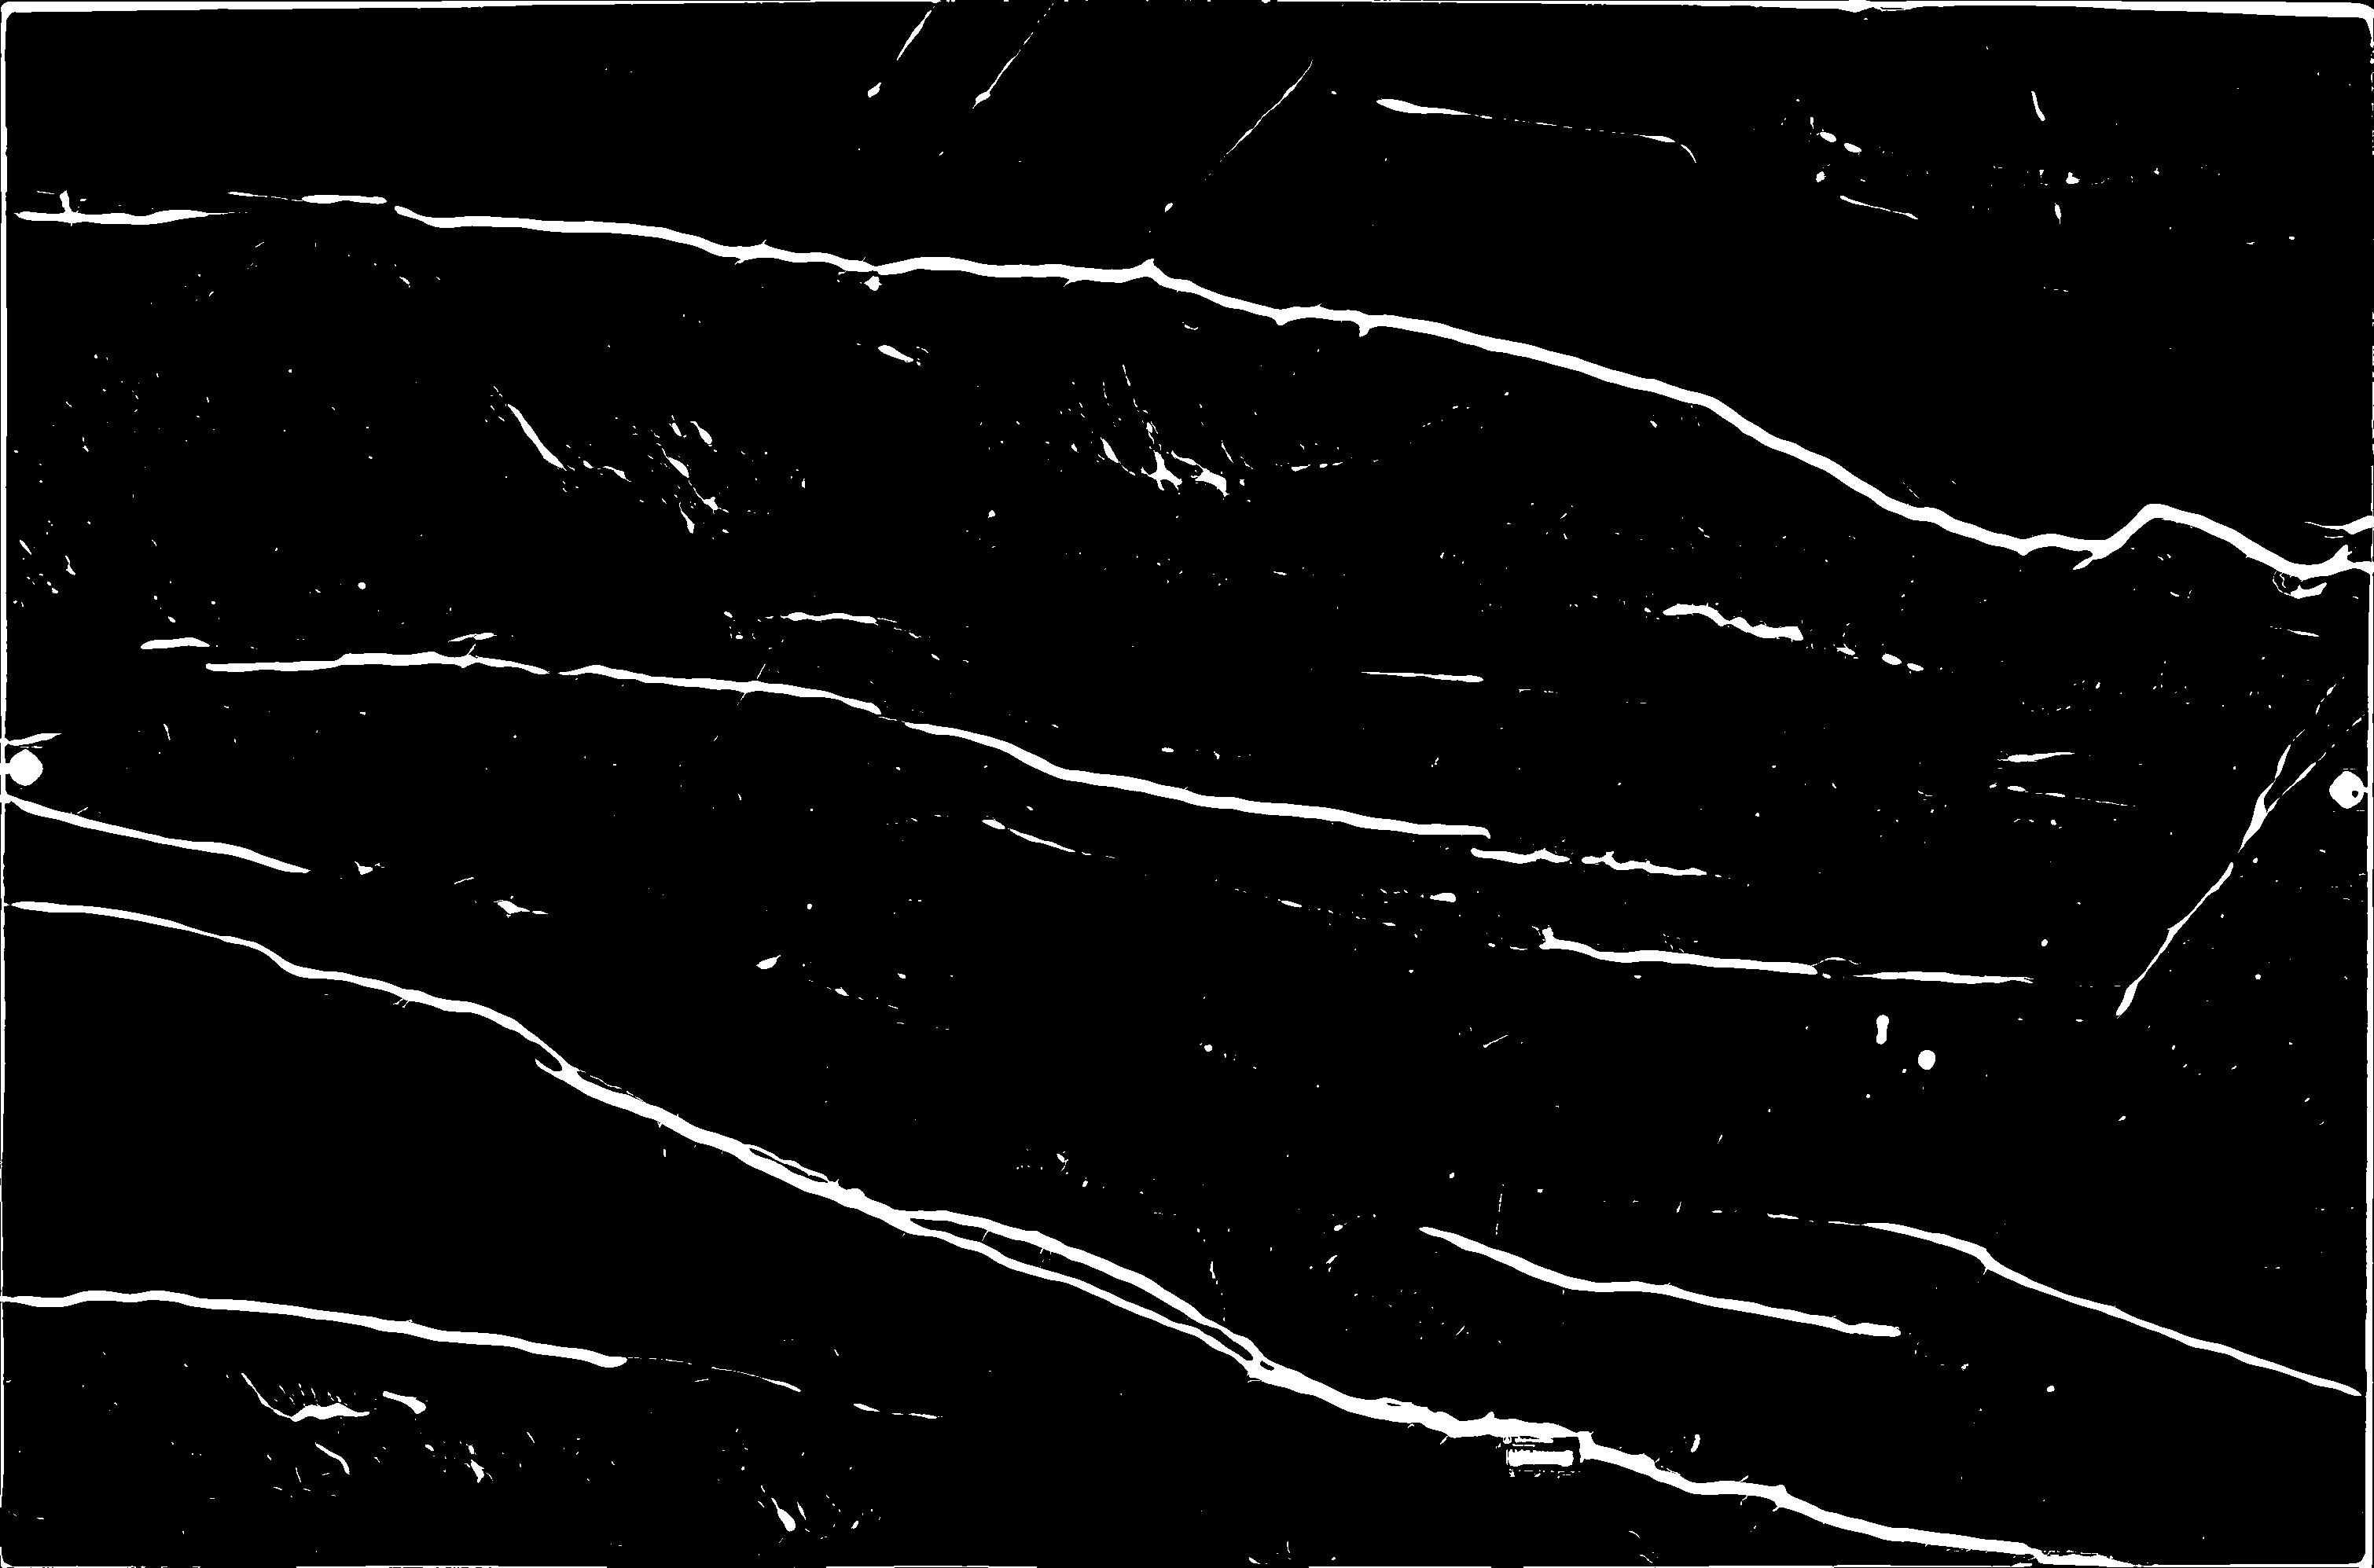
\includegraphics[width=.7\textwidth]{slabs/meijering/meije}
        \\
        \includegraphics[width=.7\textwidth]{slabs/canny/canny_origin}
        \caption{Meijering \& Contrast filter}\label{fig:meij_compare}
    \end{figure}
    In figure~\ref*{fig:meij_compare} is possible to see the result of the Meijering \& Contrast filter.
    \item \textbf{HED}\footcite{paper:hed}: this method is based on the HED algorithm.
    The HED algorithm is an edge detection algorithm that uses a deep neural network to detect the edges in images.
    The algorithm consists of 3 steps:
    \begin{enumerate}
        \item Pre-trained network: the pre-trained network is used to extract the features from the image;
        \item Multi-scale: the multi-scale algorithm is used to extract the edges from the features;
        \item Edge linking: the edges are linked using the Canny algorithm.
    \end{enumerate}
    \begin{figure}[H]
        \centering
        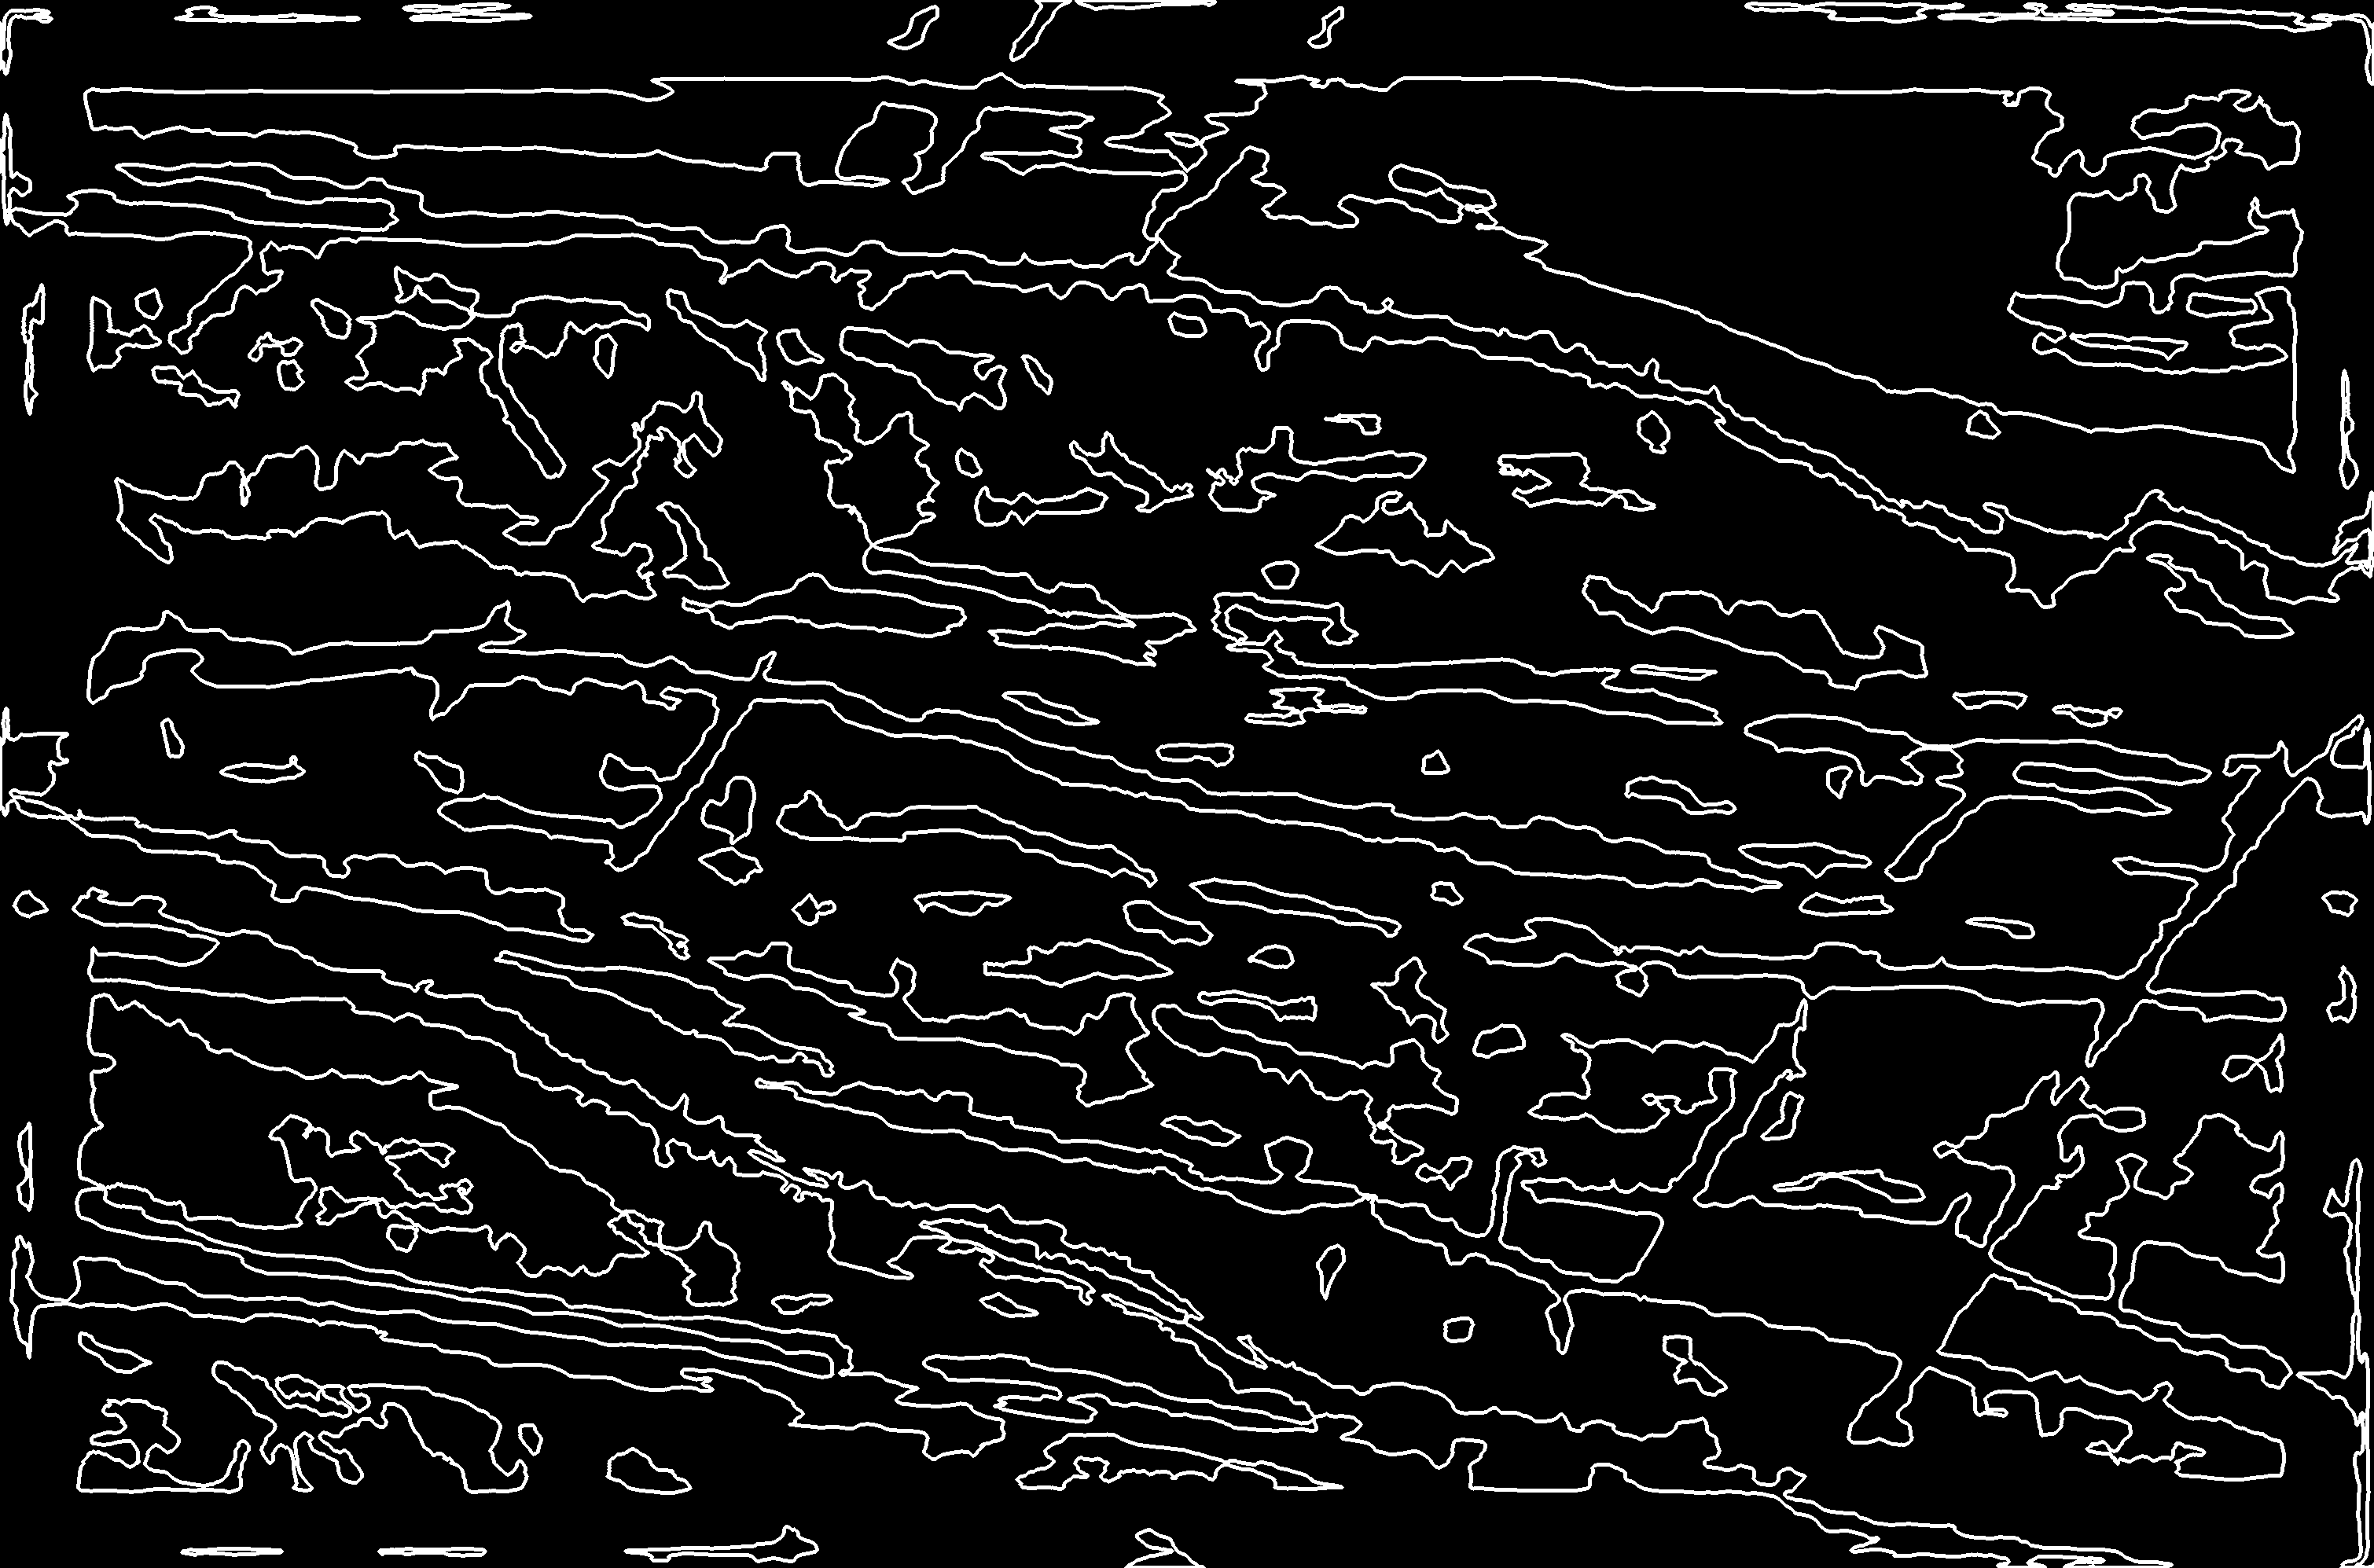
\includegraphics[width=.7\textwidth]{slabs/hed/hed}
        \\
        \includegraphics[width=.7\textwidth]{slabs/canny/canny_origin}
        \caption{HED}\label{fig:hed_compare}
    \end{figure}
    In figure~\ref*{fig:hed_compare} is possible to see the result of the HED algorithm.
\end{itemize}
\subsubsection{Milestone:}
At the end of the period the results showed that the best methods were the Meijering \& Contrast filter and the Canny Edge Detection.
HED was discarded because it was too slow and the results were not better than the other methods, many times it generates a lot of noise in the image (Random lines).
The two `winners' were able to extract the vein from the image, in an excellent way keeping in mind that was an unsupervised method.
\subsubsection{Improvements:}
One of the possible improvements is to use a supervised method to extract the vein.
This method will be more accurate than the non supervised method, because it will be trained to extract the vein.
But it requires a lot of time and hand labeled images to train the model.
\subsection{Fourth Period:}
This period was dedicated to the training of the network.
The network used was a pix2pix network, that is a network that uses a \gls{cgang} to generate images.
The training of the network was done using the dataset created in the previous periods and the hardware provided by the company. (See~\ref{subsec:hardware})
During this time different configuration of the network were tested, to find the best one, tweking the hyperparameters of the network.
The exact configuration of the network will be explained in chapter~\ref{cap:design-coding}.
\subsubsection{Milestone:}
At the end of the period the network was able to generate images of slabs, with a good variance of colors and textures (See~\ref*{fig:gen-images}).
%list of img generated
\begin{figure}
    \centering
    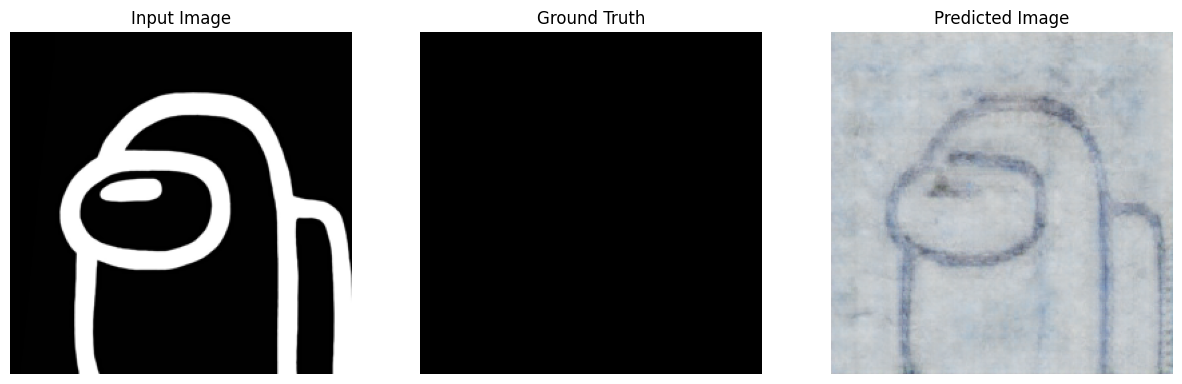
\includegraphics[width=.7\textwidth]{slabs/generated/amogus}
    \\
    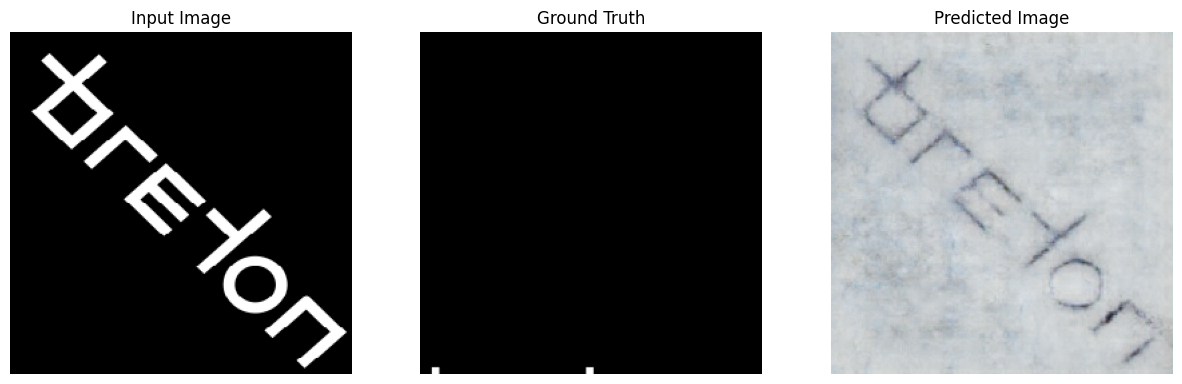
\includegraphics[width=.7\textwidth]{slabs/generated/breton}
    \\
    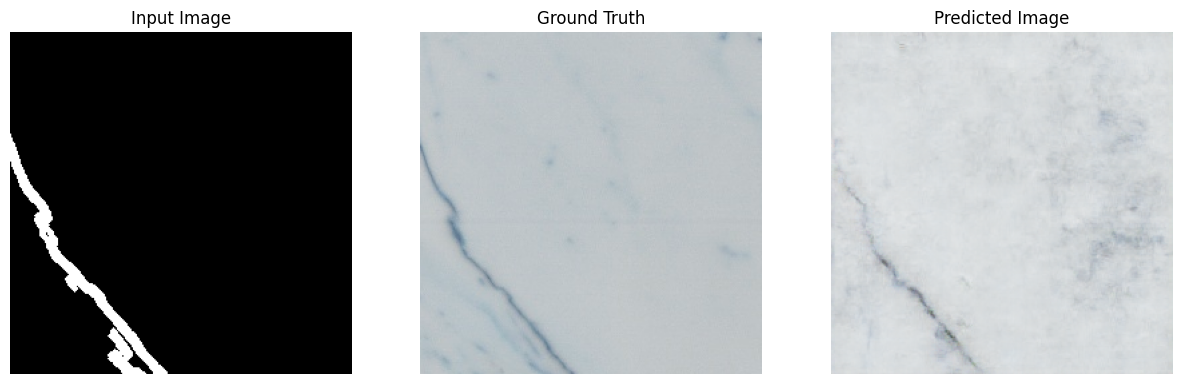
\includegraphics[width=.7\textwidth]{slabs/generated/slab}
    \caption{Generated images}\label{fig:gen-images}
\end{figure}
    %\chapter{Analisi dei requisiti}
\label{cap:analisi-requisiti}

\intro{Breve introduzione al capitolo}\\

\section{Casi d'uso}

Per lo studio dei casi di utilizzo del prodotto sono stati creati dei diagrammi.
I diagrammi dei casi d'uso (in inglese \emph{Use Case Diagram}) sono diagrammi di tipo \gls{uml} dedicati alla descrizione delle funzioni o servizi offerti da un sistema, così come sono percepiti e utilizzati dagli attori che interagiscono col sistema stesso.
Essendo il progetto finalizzato alla creazione di un tool per l'automazione di un processo, le interazioni da parte dell'utilizzatore devono essere ovviamente ridotte allo stretto necessario. Per questo motivo i diagrammi d'uso risultano semplici e in numero ridotto.

\begin{figure}[!h] 
    \centering 
    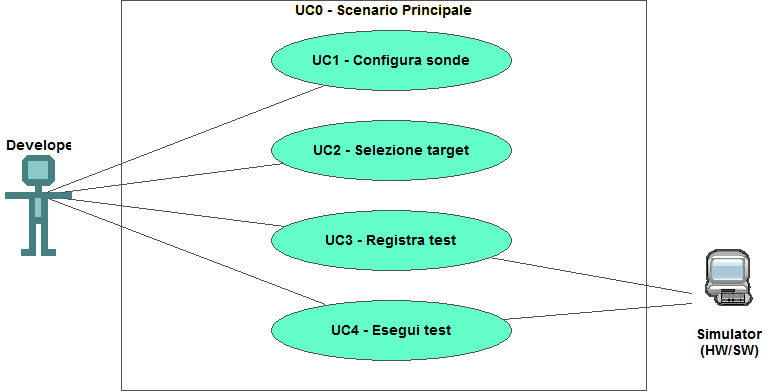
\includegraphics[width=0.9\columnwidth]{usecase/scenario-principale} 
    \caption{Use Case - UC0: Scenario principale}
\end{figure}

\begin{usecase}{0}{Scenario principale}
\usecaseactors{Sviluppatore applicativi}
\usecasepre{Lo sviluppatore è entrato nel plug-in di simulazione all'interno dell'IDE}
\usecasedesc{La finestra di simulazione mette a disposizione i comandi per configurare, registrare o eseguire un test}
\usecasepost{Il sistema è pronto per permettere una nuova interazione}
\label{uc:scenario-principale}
\end{usecase}

\section{Tracciamento dei requisiti}

Da un'attenta analisi dei requisiti e degli use case effettuata sul progetto è stata stilata la tabella che traccia i requisiti in rapporto agli use case.\\
Sono stati individuati diversi tipi di requisiti e si è quindi fatto utilizzo di un codice identificativo per distinguerli.\\
Il codice dei requisiti è così strutturato R(F/Q/V)(N/D/O) dove:
\begin{enumerate}
	\item[R =] requisito
    \item[F =] funzionale
    \item[Q =] qualitativo
    \item[V =] di vincolo
    \item[N =] obbligatorio (necessario)
    \item[D =] desiderabile
    \item[Z =] opzionale
\end{enumerate}
Nelle tabelle \ref{tab:requisiti-funzionali}, \ref{tab:requisiti-qualitativi} e \ref{tab:requisiti-vincolo} sono riassunti i requisiti e il loro tracciamento con gli use case delineati in fase di analisi.

\newpage

\begin{table}%
\caption{Tabella del tracciamento dei requisti funzionali}
\label{tab:requisiti-funzionali}
\begin{tabularx}{\textwidth}{lXl}
\hline\hline
\textbf{Requisito} & \textbf{Descrizione} & \textbf{Use Case}\\
\hline
RFN-1     & L'interfaccia permette di configurare il tipo di sonde del test & UC1 \\
\hline
\end{tabularx}
\end{table}%

\begin{table}%
\caption{Tabella del tracciamento dei requisiti qualitativi}
\label{tab:requisiti-qualitativi}
\begin{tabularx}{\textwidth}{lXl}
\hline\hline
\textbf{Requisito} & \textbf{Descrizione} & \textbf{Use Case}\\
\hline
RQD-1    & Le prestazioni del simulatore hardware deve garantire la giusta esecuzione dei test e non la generazione di falsi negativi & - \\
\hline
\end{tabularx}
\end{table}%

\begin{table}%
\caption{Tabella del tracciamento dei requisiti di vincolo}
\label{tab:requisiti-vincolo}
\begin{tabularx}{\textwidth}{lXl}
\hline\hline
\textbf{Requisito} & \textbf{Descrizione} & \textbf{Use Case}\\
\hline
RVO-1    & La libreria per l'esecuzione dei test automatici deve essere riutilizzabile & - \\
\hline
\end{tabularx}
\end{table}%

    \chapter{Design and coding}
\label{cap:design-coding}

\intro{In this chapter we will describe the design and coding of the project.
We will start by describing the technologies and tools used, then we will
describe the software life cycle, the design and the design patterns used and
finally we will describe the coding phase.}


\section{Technology and tools}
\label{sec:technology-tools}

In the following sections we will describe the technologies and tools used in
the project.
\subsection*{Python}
\label{subsec:python}
Python is a programming language that lets you work quickly and integrate
systems more effectively. It is a high-level programming language, with
applications in numerous areas, including web programming, scripting, scientific
computing, and artificial intelligence. It is very popular and used by many
companies, such as Google, Facebook, Instagram, Spotify, Netflix, Dropbox, and
many others. It is also used in the development of many open source projects,
such as Blender, GIMP, Inkscape, and many others. It is a very versatile
language, with a very large community and a very large number of libraries
available. It is also a very simple language to learn, with a very simple
syntax, which makes it very readable and easy to understand. It is also a
language that is constantly evolving, with new versions released every year,
which makes it always up to date and with the latest technologies.

\subsection*{CUDA}
\label{subsec:cuda}
CUDA is a parallel computing platform and programming model developed by NVIDIA
for general computing on graphical processing units (GPUs). With CUDA, developers
are able to dramatically speed up computing applications by harnessing the power
of GPUs. In GPU-accelerated applications, the sequential part of the workload
runs on the CPU – which is optimized for single-threaded performance – while the
compute intensive portion of the application runs on thousands of GPU cores in
parallel. When using CUDA, developers program in popular languages such as C,
C++, Fortran, Python and MATLAB and express parallelism through extensions in
the form of a few basic keywords.

\subsection*{CuDNN}
\label{subsec:cudnn}
The NVIDIA CUDA® Deep Neural Network library (cuDNN) is a GPU-accelerated library
of primitives for deep neural networks. cuDNN provides highly tuned
implementations for standard routines such as forward and backward convolution,
pooling, normalization, and activation layers. cuDNN is part of the NVIDIA Deep
Learning SDK.

\subsection*{ML libraries}
\label{subsec:mllib}
\subsubsection*{TensorFlow}
\label{subsubsec:tensorflow}
TensorFlow is an end-to-end open source platform for machine learning. It has a
comprehensive, flexible ecosystem of tools, libraries and community resources
that lets researchers push the state-of-the-art in ML and developers easily
build and deploy ML powered applications.
\subsubsection*{PyTorch}
\label{subsubsec:pytorch}
PyTorch is an open source machine learning library based on the Torch library,
used for applications such as computer vision and natural language processing,
primarily developed by Facebook's AI Research lab (FAIR). It is free and open
source software released under the Modified BSD license. Although the Python
interface is more polished and the primary focus of development, PyTorch also
has a C++ interface.
\subsubsection*{Keras}
\label{subsubsec:keras}
Keras is a high-level neural networks \gls{apig}, written in Python and capable of
running on top of TensorFlow, CNTK, or Theano. It was developed with a focus on
enabling fast experimentation. Being able to go from idea to result with the
least possible delay is key to doing good research.
\subsubsection*{OpenCV}
\label{subsubsec:opencv}
OpenCV (Open Source Computer Vision Library) is an open source computer vision
and machine learning software library. OpenCV was built to provide a common
infrastructure for computer vision applications and to accelerate the use of
machine perception in the commercial products. Being a BSD-licensed product,    
OpenCV makes it easy for businesses to utilize and modify the code. The library
has more than 2500 optimized algorithms, which includes a comprehensive set of
both classic and state-of-the-art computer vision and machine learning
algorithms. These algorithms can be used to detect and recognize faces, identify
objects, classify human actions in videos, track camera movements, track moving
objects, extract 3D models of objects, produce 3D point clouds from stereo
cameras, stitch images together to produce a high resolution image of an entire
scene, find similar images from an image database, remove red eyes from images
taken using flash, follow eye movements, recognize scenery and establish markers
to overlay it with augmented reality, etc. OpenCV has more than 47 thousand
people of user community and estimated number of downloads exceeding 18 million.
The library is used extensively in companies, research groups and by governmental
bodies.
\subsection*{GANs Models}
\label{subsec:gans-models}
\subsubsection*{Pix2Pix}\footcite{paper:pix2pix}
\label{subsubsec:pix2pix}
Pix2Pix is a Generative Adversarial Network, or \gls{gang}, model designed for general
purpose image-to-image translation. The model was trained and evaluated on a
large dataset of paired images from the \textit{Berkeley Segmentation Dataset
and Benchmark} and demonstrates a capability to generate plausible synthetic
images for a variety of image-to-image translation tasks, such as converting
daylight images to night.

\subsubsection*{ESRGAN}\footcite{paper:esrgan}
\label{subsubsec:esrgan}
ESRGAN is an enhanced version of the \gls{esrgang} model, which is a Generative
Adversarial Network, or \gls{gang}, model designed for general purpose
image-to-image translation. The model was trained and evaluated on a large
dataset of paired images from the DIV2K dataset and demonstrates a capability to
generate plausible synthetic images for a variety of image-to-image translation
tasks, such as converting low resolution images to high resolution.

\subsubsection*{StyleGAN}
\label{subsubsec:stylegan}
StyleGAN is a Generative Adversarial Network, or \gls{gang}, model designed for
general purpose image generation. The model was trained and evaluated on a large
dataset of unpaired images from the Flickr-Faces-HQ dataset and demonstrates a
capability to generate plausible synthetic images for a variety of image
generation tasks, such as generating realistic human faces.

\subsection*{Tools}
\label{subsec:tools}
\subsubsection*{Visual Studio Code}
\label{subsubsec:vscode}
Visual Studio Code is a free source-code editor made by Microsoft for Windows,
Linux and macOS. Features include support for debugging, syntax highlighting,
intelligent code completion, snippets, code refactoring, and embedded Git.
\subsubsection*{Git}
\label{subsubsec:git}
Git is a distributed version-control system for tracking changes in source code
during software development. It is designed for coordinating work among
programmers, but it can be used to track changes in any set of files. Its goals
include speed, data integrity, and support for distributed, non-linear
workflows.
\subsubsection*{GitHub}
\label{subsubsec:github}
GitHub is a global company that provides hosting for software development
version control using Git. It is a subsidiary of Microsoft, which acquired the
company in 2018 for \$7.5 billion. It offers all of the distributed version
control and source code management (SCM) functionality of Git as well as adding
its own features. It provides access control and several collaboration features
such as bug tracking, feature requests, task management, and wikis for every
project.
\subsubsection*{GIMP}
\label{subsubsec:gimp}
GIMP is a free and open-source raster graphics editor used for image retouching
and editing, free-form drawing, converting between different image formats, and
more specialized tasks.
\subsubsection*{Webex}
\label{subsubsec:webex}
Webex is a video conferencing software developed by Cisco Systems. It is a
cloud-based software that provides video conferencing, online meetings,
screen-sharing, and webinars. It has a free version that allows up to 100
participants, with a 50-minute time restriction. The paid version starts at
\$13.50/month and allows up to 200 participants and unlimited meeting time.
\subsubsection*{Outlook}
\label{subsubsec:outlook}
Outlook is a personal information manager software system from Microsoft,
available as a part of the Microsoft Office suite. Primarily an email
application, it also includes a calendar, task manager, contact manager,
note taking, journal, and web browsing.

\subsection*{Hardware}
\label{subsec:hardware}
All the hardware used for the development of this project was provided by the
company. The hardware used for the development of this project is listed below: \\
\begin{itemize}
    \item \textbf{DELL Precision 7670}
    \begin{itemize}
        \item \textbf{CPU}: Intel Core i7-12850HX
        \item \textbf{GPU}: NVIDIA Quadro RTX A2000 8GB GDDR6
        \item \textbf{RAM}: 32GB DDR4
        \item \textbf{Storage}: 512GB NVMe SSD
        \item \textbf{OS}: Windows 10 Pro 64-bit
    \end{itemize}
    \item \textbf{DELL Precision 7520}
    \begin{itemize}
        \item \textbf{CPU}: Intel Core i7-6820HQ
        \item \textbf{GPU}: NVIDIA Quadro M2200 4GB GDDR5
        \item \textbf{RAM}: 16GB DDR4
        \item \textbf{Storage}: 512GB NVMe SSD
        \item \textbf{OS}: Windows 10 Pro 64-bit
    \end{itemize}
\end{itemize}
\section{Ciclo di vita del software}
\label{sec:ciclo-vita-software}

\section{Progettazione}
\label{sec:progettazione}

\subsubsection{Namespace 1} %**************************
Descrizione namespace 1.

\begin{namespacedesc}
    \classdesc{Classe 1}{Descrizione classe 1}
    \classdesc{Classe 2}{Descrizione classe 2}
\end{namespacedesc}


\section{Design Pattern utilizzati}

\section{Codifica}

    \chapter{Verification and validation}\label{cap:verification-validation}
\intro{
    In this chapter we will discuss the verification and validation process of the trained model.
    We will discuss the metrics used to evaluate the model and the results obtained.
}
\section{Metrics}\label{sec:metrics}
\subsection{Loss function}
According to the pix2pix paper \footcite{paper:pix2pix}, the loss function used is a combination of a conditional GAN loss and a L1 loss.
In a general CGAN the objective function is defined as:
\begin{equation}
    \label{eq:cgan-loss}
    L_{cGAN}(G, D) = \mathbb{E}_{x,y}[\log D(x, y)] + \mathbb{E}_{x,z}[\log(1 - D(x, G(x, z)))]
\end{equation}
here $G$ tries to minimize this function against an adversarial $D$ that tries to maximize it.
To assess the significance of conditioning the discriminator, we also compare it to an unconditional variant where the discriminator does not have access to the input x. 
The loss function for this unconditional variant can be expressed as:
\begin{equation}
    \label{eq:cgan-loss-uncond}
    L_{cGAN}(G, D) = \mathbb{E}_{x,y}[\log D(y)] + \mathbb{E}_{x,z}[\log(1 - D(G(x, z)))]
\end{equation}
Previous studies have shown the advantages of incorporating a traditional loss, such as L2 distance \footcite{paper:DPathakCVPR16}, alongside the GAN objective. 
While the discriminator's role remains unchanged, the generator is not only responsible for fooling the discriminator but also for producing outputs that closely resemble the ground truth in terms of L2 similarity. 
Additionally, we explore an alternative option by employing L1 distance instead of L2, as L1 promotes reduced blurring:
The L1 loss for the generator can be defined as:
\begin{equation}
    \label{eq:l1-loss}
    L_{L1}(G) = \mathbb{E}_{x,y,z}\left[\left\|y - G(x, z)\right\|_1\right]
\end{equation}
Our ultimate objective is to find the optimal generator G that minimizes the loss function while simultaneously maximizing the performance of the discriminator D. 
This objective can be represented by the equation:
\begin{equation}
    G^* = \arg \min_G \max_D \left( L_{cGAN}(G, D) + \lambda L_{L1}(G) \right)
\end{equation}
In previous conditional GAN approaches, the inclusion of Gaussian noise z alongside the input x was employed to prevent deterministic outputs and allow for the modeling of diverse distributions. 
However, in our experiments, this strategy was found to be ineffective as the generator learned to ignore the noise, aligning with the findings of Mathieu et al. \footcite{paper:MMathieuICLR16}. 
Instead, in our final models, we introduce noise through the use of dropout applied to multiple layers of the generator during both training and testing. 
Despite the presence of dropout noise, we observe only minor stochasticity in the generated outputs. 
The development of conditional GANs that can produce highly stochastic outputs, capturing the full entropy of the conditional distributions they model, remains an open and important question for future research.
%\subsection{Evaluation metrics}
%\subsubsection{\gls{FIDG} score}
%The Fréchet Inception Distance (\gls{FIDG}\glsfirstoccur) score is a widely used metric for evaluating the quality of generated images in the field of generative adversarial networks (GANs) introduced by Martin Heusel et al. \footcite{paper:heusel2017gans}. 
%It measures the similarity between the distribution of real images and the distribution of generated images by comparing their feature representations extracted from a pre-trained Inception-v3 network. 
%A lower FID score indicates better similarity between the two distributions, suggesting higher-quality generated images that resemble the real data more closely. 
%The FID score takes into account both the quality and diversity of generated images, making it a valuable metric for assessing the performance of GAN models. 
%It provides a quantitative measure that complements visual inspection and subjective evaluation, enabling researchers to objectively compare and analyze different GAN architectures and training strategies.
%The \gls{FIDG} score is defined as:
%\begin{equation}
%    \label{eq:fid-score}
%    \text{FID}(p, q) = \|\mu_p - \mu_q\|^2 + \text{Tr}(\Sigma_p + \Sigma_q - 2(\Sigma_p\Sigma_q)^{1/2})
%\end{equation}
%Where:
%\begin{itemize}
%    \item $\mu_p$ and $\mu_q$ are the mean vectors of the real and generated images respectively.
%    \item $\Sigma_p$ and $\Sigma_q$ are the covariance matrices of the real and generated images respectively.
%    \item \text{Tr} is the trace operator.
%    \item $\|\cdot\|$ is the Euclidean norm.
%\end{itemize}
%\subsubsection{Inception score}

\section{Results}\label{sec:results}
\subsection{Evaluation metrics}
During the training process, the evaluation metrics were calculated every 100 epochs.
For get a more accurate result, the evaluation metrics were calculated using the same couple of image-mask for each epoch, generating ten images for each epoch.
Each generated image was compared with the corresponding real image.
\subsubsection{FID score}
During the training process, the FID score was calculated every 100 epochs. 
%Table for compare FID score
\begin{table}[H]
    \centering
    \begin{tabular}{|c|c|c|}
        \hline
        \textbf{Model} & \textbf{FID score} & \textbf{Epoch} \\
        \hline
        \hline
        \textbf{M1} & 32,98 & 100 \\
        \hline
        \textbf{M2} & 26,42 & 200 \\
        \hline
        \textbf{M3} & 25,39 & 300 \\
        \hline
        \textbf{M4} & 22,29 & 400 \\
        \hline
        \textbf{M5} & 22,29 & 500 \\
        \hline
        \textbf{M6} & 22,29 & 600 \\
    \end{tabular}
    \caption{Mean FID score for each model}\label{tab:fid-score}
\end{table}
According to the results obtained, the best model is the \textbf{M3} model.
\subsubsection{Inception score}
During the training process, the Inception score was calculated every 100 epochs.
%Table for compare Inception score
\begin{table}[H]
    \centering
    \begin{tabular}{|c|c|c|}
        \hline
        \textbf{Model} & \textbf{Inception score} & \textbf{Epoch} \\
        \hline
        \hline
        \textbf{M1} & 0,6589 & 100 \\
        \hline
        \textbf{M2} & 0,7461 & 200 \\
        \hline
        \textbf{M3} & 0,7596 & 300 \\
        \hline
        \textbf{M4} & 0,7435 & 400 \\
        \hline
        \textbf{M5} & 0,7005 & 500 \\
        \hline
        \textbf{M6} & 0,7362 & 600 \\
    \end{tabular}
    \caption{Mean Inception score for each model}\label{tab:inception-score}
\end{table}
According to the results obtained, the best model is the \textbf{M3} model.

\section{Different Network Configurations}\label{sec:different-network-configurations}
During the training process, a problem was encountered where the image quality started to deteriorate after a certain number of epochs. Upon analyzing the loss curve, it became evident that the discriminator's loss was decreasing rapidly. 
This led me to believe that the discriminator was learning features at a faster rate than the generator.
To address this issue, I made several adjustments to the network's hyper-parameters:
\begin{itemize}
    \item Initially, I started training with the standard configuration and disabled discriminator training after 140k steps to prevent it from surpassing the generator's performance. Unfortunately, this modification resulted in even worse outcomes.
    \item I also experimented with disabling dropout on the three layers, suspecting that it might be responsible for the poor results and adversely affecting the model.
    \item Another attempt involved training the model for 150k steps and reducing the discriminator's learning rate to 0.0001, instead of completely disabling its training. However, this approach also yielded unsatisfactory results.
\end{itemize}
Ultimately, it was discovered that the issue did not lie with the network's hyper-parameters, but rather with the training dataset itself.
The training dataset posed a challenge as it was created through an unsupervised process, resulting in the inclusion of numerous low-quality images. Some of these images contained only white spots instead of a complete line representing a vein, which affected the overall image quality. Recognizing this issue, I took steps to address it by removing such problematic images from the dataset.

As the training progressed and these flawed images were eliminated, the image quality gradually improved with each epoch. This suggests that the removal of these specific images played a crucial role in enhancing the overall performance and realism of the generated images.
    \chapter{Conclusion}\label{cap:conclusions}
\intro{
    In this chapter we will present the conclusions of our work, the results obtained and the future developments of the project.
}
\section{Goals achieved}
In the following table we will show the goals achieved and the ones that are still in progress. (Refer to table~\ref{tab:goals} for the meaning of the acronyms)
\begin{table}[H]
    \caption{Reached Goals}\label{tab:reach-goals}
    \centering
    \begin{tabularx}{\textwidth}{|c|X|}
        \hline
        \textbf{Code} & \textbf{Status}\\
        \hline
        M1 & Achieved\\
        \hline
        M2 & Achieved\\
        \hline
        M3 & Achieved\\
        \hline
        D1 & Achieved\\
        \hline
        D2 & Not Achieved\\
        \hline
        D3 & Achieved\\
        \hline
        O1 & Achieved\\
        \hline
        O2 & Partially Achieved\\
        \hline
    \end{tabularx}
\end{table}
All the goals marked as achieved are fully implemented and tested.
\textbf{D2} was tested but the results were not satisfactory, so it was decided to not implement it.
\textbf{O2} was partially implemented, the model and the technologies are too young to be used in a manufacturing production environment.
\section{Hourly summary}
As per the initial work plan, a total of 320 hours were allocated for the project, with an intentional overestimation of hourly commitments to account for potential absences or unforeseen circumstances. 
The purpose of this buffer was to ensure that the project could be completed comfortably within the allocated time frame.
Upon completion of the project, it was found that the actual total hours invested in the project amounted to 300 hours. 
This indicates that the project was completed within the expected time frame, demonstrating a commendable consistency between the planned and actual hours spent.
The adherence to the projected hour count is indicative of effective project management and efficient utilization of resources. 
The slight underestimation of hours compared to the initial estimate further highlights the successful management of time and effort throughout the project duration.
\section{Acquired knowledge}
During the course of the project, I had the opportunity to acquire valuable managerial and interpersonal skills while working in a collaborative research team comprising three individuals. 
Additionally, I delved into fields of AI that were previously unfamiliar to me, gaining comprehensive knowledge not only about AI in general but also, in particular, about Generative Adversarial Networks (GANs).

One of the significant areas of growth was in the realm of project management. Collaborating with team members allowed me to enhance my ability to coordinate tasks, set goals, and allocate resources effectively. 
I also developed strong communication and teamwork skills through regular interactions, discussions, and brainstorming sessions. 
This experience highlighted the importance of clear and concise communication, active listening, and the ability to work harmoniously towards a common objective.

In terms of technical knowledge, I embarked on an exploration of AI fields that were previously unfamiliar to me. 
This journey broadened my understanding of AI principles, methodologies, and techniques. 
More specifically, I gained in-depth knowledge about Generative Adversarial Networks (GANs) and their applications in various domains. 
This encompassed comprehending the underlying architecture, training procedures, and optimization techniques related to GANs.

Furthermore, I expanded my expertise in Python libraries specifically tailored for computer vision and AI applications. 
Through hands-on experience, I became proficient in utilizing popular libraries such as TensorFlow, PyTorch, and OpenCV.\@
These libraries proved instrumental in implementing computer vision algorithms and working with AI models efficiently.

In summary, this project provided me with valuable insights and knowledge in both managerial and technical domains. 
The collaborative research environment fostered the development of essential interpersonal skills, while the exploration of unfamiliar AI fields and the utilization of Python libraries enhanced my technical proficiency. 
The acquired knowledge and skills from this project will undoubtedly contribute to my future endeavors in the field of AI and beyond.
\section{Personal evaluation.}
My internship experience has been truly invaluable and has provided me with a multitude of learning opportunities and personal growth. 
Throughout the duration of the internship, I have had the chance to work in a professional setting, applying the knowledge and skills I acquired during my studies.

One aspect of the internship that I found particularly rewarding was the exposure to real-world scenarios and challenges. This allowed me to bridge the gap between theory and practice, gaining a deeper understanding of how concepts and principles are applied in a professional context. 
The hands-on experience has enhanced my problem-solving abilities and critical thinking skills, enabling me to approach tasks with a more practical and solution-oriented mindset.

Moreover, the internship provided me with a chance to collaborate with a diverse team of professionals. This collaborative environment allowed me to learn from others, exchange ideas, and contribute to meaningful projects. 
Working alongside experienced colleagues has not only expanded my technical knowledge but has also helped me refine my interpersonal skills such as effective communication, teamwork, and adaptability.

also appreciated the mentorship and guidance provided by my supervisor throughout the internship. 
Their support and feedback have been instrumental in my growth and development. They provided valuable insights, challenged me to think outside the box, and encouraged me to take ownership of my work. 
This guidance has not only enhanced my technical skills but has also boosted my confidence in tackling complex tasks and projects.

In terms of personal growth, this internship has helped me develop a greater sense of professionalism and work ethic. It has instilled in me a strong sense of responsibility, time management, and the importance of meeting deadlines. 
The experience has also reinforced my passion for the field and has motivated me to continue exploring and expanding my knowledge beyond the internship.

Overall, my internship experience has been incredibly rewarding. It has provided me with practical skills, industry exposure, and personal growth opportunities. 
I am grateful for the chance to apply my knowledge, collaborate with professionals, and learn from experienced mentors. The lessons and experiences gained during this internship will undoubtedly have a lasting impact on my future career endeavors.

    %\appendix
    %\chapter{Appendix A}

\epigraph{Quote}{Author}


    \backmatter
    \printglossary[type=\acronymtype, title=Acronyms and abbreviations, toctitle=Acronyms and abbreviations]
    \printglossary[type=main, title=Glossary, toctitle=Glossary]

    \cleardoublepage
\chapter{Bibliography}

\nocite{*}

% Print book bibliography
\printbibliography[heading=subbibliography,title={Book bibliography},type=book]

% Print site bibliography
\printbibliography[heading=subbibliography,title={Web-Site bibliography},type=online]

\end{document}
